\section{Mức 7,8 điểm}
\Opensolutionfile{ans}[ans/CD10/Muc_7_8]
\setcounter{dang}{0}
\setcounter{ex}{0}
\begin{dang}
	{Cạnh bên vuông góc với đáy}
\end{dang}
\begin{ex}[Đề Minh Họa 2021]%[2H1K3-2]
Cho hình chóp $ S.ABC$ có đáy $ ABC$ là tam giác đều cạnh $ a$, cạnh bên $ SA$ vuông góc với mặt phẳng đáy, góc giữa $ SA$và mặt phẳng $ (SBC)$ bằng $45^0$ (tham khảo hình bên). Thể tích khối chóp $ S.ABC$ bằng
\begin{center}
    \begin{tikzpicture}[>=stealth, line join=round, line cap = round]
        \def\a{-1.5} \def\b{2} \def\c{3} \def\x{5}
\coordinate (A) at (0,0);
\coordinate (S) at (0,\c);
\coordinate (B) at (\b,\a);
\coordinate (C) at (\x,0);
        \draw (S) node[left]{$S$} -- (A) node[left]{$A$} -- (B) node[below]{$B$} -- (C) node[right]{$S$} -- (S) -- (B);
        \draw[dashed] (A) -- (C);
\fill (A)circle(1pt) 
(B)circle(1pt) 
(C)circle(1pt) 
(S)circle(1pt) ;
    \end{tikzpicture}
\end{center}
\choice
{\True $\dfrac{a^3}{8}$}
{$\dfrac{3a^3}{8}$}
{$\dfrac{\sqrt{3}{a^3}}{12}$}
{$\dfrac{a^3}{4}$}
\loigiai{
\begin{center}
    \begin{tikzpicture}[>=stealth, line join=round, line cap = round]
        \def\a{-1.5} \def\b{2} \def\c{3} \def\x{5}
\coordinate (A) at (0,0);
\coordinate (S) at (0,\c);
\coordinate (B) at (\b,\a);
\coordinate (C) at (\x,0);
\coordinate (M) at ($(B)!0.5!(C)$);
\coordinate (H) at ($(S)!0.4!(M)$);
        \draw (S) node[left]{$S$} -- (A) node[left]{$A$} -- (B) node[below]{$B$} -- (C) node[right]{$C$} -- (S) -- (B);
        \draw[dashed] (A) -- (C);
        \draw[dashed] (A) -- (M) node[right]{$M$};
        \draw[dashed] (A) -- (H) node[right]{$H$};
        \draw (S) -- (M);
        \fill (A)circle(1pt) 
(B)circle(1pt) 
(C)circle(1pt) 
(S)circle(1pt)
(M)circle(1pt) 
(H)circle(1pt);
    \end{tikzpicture}
\end{center}
Gọi $ M$ là trung điểm $ BC$ thì $ AM\perp BC$ và $ SA\perp BC$ nên $ BC\perp (SAM).$\\
Kẻ $ AH\perp SM$ tại $ H$ thì $ AH\perp\left(SBC\right)$. Suy ra góc giữa $ SA$và mặt phẳng $ (SBC)$ bằng $\widehat{ASH}=\widehat{ASM}=45^\circ $. Do đó, $\Delta SAM$ vuông cân ở $ A$ và $ SA=AM=\dfrac{a\sqrt{3}}{2}.$\\
Suy ra $V_{S.ABC}=\dfrac{1}{3}\cdot\dfrac{a\sqrt{3}}{2}\cdot\dfrac{a^2\sqrt{3}}{4}=\dfrac{a^3}{8}.$}
\end{ex}
%
\begin{ex}[Mã 105 2017]%[2H1K3-2]
Cho khối chóp $S.ABCD$ có đáy là hình vuông cạnh $ a$, $ SA$ vuông góc với đáy và khoảng cách từ $ A$ đến mặt phẳng $\left(SBC\right)$ bằng $\dfrac{a\sqrt{2}}{2}$. Tính thể tích của khối chóp đã cho.
\choice
{\True $\dfrac{a^3}{3}$}
{$a^3$}
{$\dfrac{\sqrt{3}{a^3}}{9}$}
{$\dfrac{a^3}{2}$}
\loigiai
{
\begin{center}
    \begin{tikzpicture}[>=stealth, line join=round, line cap = round]
        \def\a{-1.5} \def\b{2} \def\c{3} \def\x{5}
\coordinate (S) at (0,\c);
\coordinate (A) at (0,0);
\coordinate (B) at (-\b,\a);
\coordinate (C) at (\x,0);
\coordinate (D) at ($(B) + (C)$);
\coordinate (H) at ($(S)!0.4!(B)$);
        \draw (S) node[left]{$S$} -- (B) node[below]{$B$} -- (D) node[below]{$D$} -- (C) node[right]{$C$} -- (S) -- (D);
        \draw[dashed] (H) node[left]{$H$} -- (A) node[above right]{$A$} -- (C);
        \draw[dashed] (B) -- (A) -- (S);
\fill (A)circle(1pt) 
(B)circle(1pt) 
(C)circle(1pt) 
(S)circle(1pt)
(D)circle(1pt) 
(H)circle(1pt);
    \end{tikzpicture}
\end{center}
Ta có $ BC\perp AB,BC\perp SA\Rightarrow BC\perp AH$. Kẻ $ AH\perp SB\Rightarrow AH\perp\left(SBC\right)$.\\
Suy ra $ d\left(A;\left(SBC\right)\right)=AH=\dfrac{a\sqrt{2}}{2}$.\\
Tam giác $ SAB$ vuông tại $ A$ có: $\dfrac{1}{A{H^2}}=\dfrac{1}{S{A^2}}+\dfrac{1}{A{B^2}}\Rightarrow SA=a$.\\
Vậy $V_{SABCD}=\dfrac{1}{3}SA.S_{ABCD}=\dfrac{a^3}{3}$.}
\end{ex}
%
\begin{ex}[Mã 110 2017]%[2H1K3-2]
Cho khối chóp $ S.ABCD$có đáy $ ABCD$ là hình chữ nhật, $ AB=a$, $ AD=a\sqrt{3}$, $ SA$ vuông góc với mặt phẳng đáy và mặt phẳng $\left(SBC\right)$ tạo với đáy một góc $60^o$. Tính thể tích $ V$ của khối chóp $ S.ABCD$.
\choice
{$ V=3a^3$}
{$ V=\dfrac{\sqrt{3}{a^3}}{3}$}
{\True $ V=a^3$}
{$ V=\dfrac{a^3}{3}$}
\loigiai
{
\begin{center}
    \begin{tikzpicture}[>=stealth, line join=round, line cap = round]
        \def\a{-1.5} \def\b{2} \def\c{3.5} \def\x{5}
\coordinate (S) at (0,\c);
\coordinate (A) at (0,0);
\coordinate (D) at (-\b,\a);
\coordinate (B) at (\x,0);
\coordinate (C) at ($(D) + (B)$);
        \draw (S) node[left]{$S$} -- (B) node[below]{$B$} -- (C) node[below]{$C$} -- (D) node[below]{$D$} -- (S) -- (C);
        \draw[dashed] (A) node[above=9pt, right=5pt]{$A$} -- (C);
        \draw[dashed] (A) -- (S);
        \draw[dashed] (A) -- (D) node[pos=0.5,sloped,above]{$a \sqrt{3}$};
        \draw[dashed] (A) -- (B) node[pos=0.5,sloped,above]{$a$};
        \draw[dashed] (B) -- (D);
        \draw pic[draw,blue,fill=green!50,opacity=.55,angle radius=5mm,angle eccentricity=1.7,"$60^\circ$"] {angle = S--B--A};
    \pic[draw,angle radius=3mm]{right angle=S--A--D};
    \pic[draw,angle radius=3mm]{right angle=B--A--D};
    \pic[draw,angle radius=3mm]{right angle=B--A--S};
\fill (A)circle(1pt) 
(B)circle(1pt) 
(C)circle(1pt) 
(S)circle(1pt)
(D)circle(1pt);

    \end{tikzpicture}
\end{center}
Ta có $S_{ABCD}=\sqrt{3}{a^2}$.\\
Vì $\left\{\begin{aligned}
&\left(SBC\right)\cap\left(ABCD\right)=BC\\ 
& BC\perp SB\subset\left(SBC\right)\\ 
& BC\perp AB\subset\left(ABCD\right)\\ 
\end{aligned}\right.\Rightarrow\widehat{\left(\left(SBC\right),\left(ABCD\right)\right)}=\widehat{\left(SB;AB\right)}=\widehat{SBA}$.\\
Vậy $\widehat{SBA}=60^o$\\
Xét tam giác vuông $ SAB$ có: $\tan{60^o}=\dfrac{SA}{AB}\Rightarrow SA=AB.\tan{60^o}=a\sqrt{3}$.\\
Vậy $V_{S.ABCD}=\dfrac{1}{3}{S_{ABCD}}.SA=\dfrac{1}{3}{a^2}\sqrt{3}.a\sqrt{3}=a^3$.}
\end{ex}
%
\begin{ex}[Mã 123 2017]%[2H1K3-2]
 Cho hình chóp $S.ABCD$ có đáy là hình vuông cạnh $ a$, $SA$ vuông góc với đáy, $SC$ tạo với mặt phẳng $\left(SAB\right)$ một góc $30^0$. Tính thể tích khối chóp $S.ABCD$ 
\choice
{$\dfrac{2a^3}{3}$}
{\True $\dfrac{\sqrt{2}{a^3}}{3}$}
{$\dfrac{\sqrt{6}{a^3}}{3}$}
{$\sqrt{2}{a^3}$}
\loigiai
{
\begin{center}
    \begin{tikzpicture}[>=stealth, line join=round, line cap = round]
        \def\a{-1.5} \def\b{2} \def\c{3} \def\x{5}
\coordinate (S) at (0,\c);
\coordinate (A) at (0,0);
\coordinate (B) at (-\b,\a);
\coordinate (D) at (\x,0);
\coordinate (C) at ($(B) + (D)$);
        \draw (S) node[left]{$S$} -- (B) node[below]{$B$} -- (C) node[below]{$C$} -- (D) node[right]{$D$} -- (S) -- (C);
        \draw[dashed] (A) node[above right]{$A$} -- (D);
        \draw[dashed] (B) -- (A) -- (S);
    \draw pic[draw,blue,fill=green!50,opacity=.5,angle radius=8mm,angle eccentricity=1.5,"$30^\circ$"] {angle = B--S--C};
\fill (A)circle(1pt) 
(B)circle(1pt) 
(C)circle(1pt) 
(S)circle(1pt)
(D)circle(1pt);
    \end{tikzpicture}
\end{center}
+) Do ABCD là hình vuông cạnh a nên: $S_{ABCD}=a^2$\\
+) Chứng minh được $ BC\perp\left(SAB\right)\Rightarrow $ góc giữa SC và (SAB) là $\widehat{CSB}=30^0$.\\
+) Đặt $ SA=x$$\Rightarrow SB=\sqrt{x^2+a^2}$. Tam giác SBC vuông tại B nên $\tan\widehat{CSA}=\tan{30^0}=\dfrac{1}{\sqrt{3}}=\dfrac{BC}{SB}$.\\
Ta được: $ SB=BC\sqrt{3}\Leftrightarrow\sqrt{x^2+a^2}=a\sqrt{3}\Rightarrow x=a\sqrt{2}$.\\
Vậy $V_{SABCD}=\dfrac{1}{3}.SA.S_{ABCD}=\dfrac{1}{3}.a\sqrt{2}.a^2=\dfrac{\sqrt{2}{a^3}}{3}$ (Đvtt).}
\end{ex}

\begin{ex}[Chuyên Vĩnh Phúc 2019]%[2H1K3-2]
 Cho hình chóp $ S.ABC$ có đáy là tam giác vuông cân tại $ C,$ cạnh bên $SA$ vuông góc với mặt đáy, biết $ AB=4\text{a},SB=6\text{a}.$ Thể tích khối chóp $ S.ABC$ là $ V.$ Tỷ số $\dfrac{a^3}{3V}$ là
\choice
{$\dfrac{\sqrt{5}}{80}$}
{\True $\dfrac{\sqrt{5}}{40}$}
{$\dfrac{\sqrt{5}}{20}$}
{$\dfrac{3\sqrt{5}}{80}$}
\loigiai
{
\begin{minipage}[ht]{0.5\textwidth}
    Ta có:\\
+ $\Delta ABC$ vuông cân tại $ C,\,AB=4\text{a}$ suy ra\\
$ AC=BC=2\text{a}\sqrt{2}$.\\
Do đó: $S_{ABC}=\dfrac{1}{2}AC.BC=4\text{a}^2$.\\
+ $SA\perp\left(ABC\right)\Rightarrow SA\perp AB\Rightarrow\Delta ABC$ vuông tại $ A$\\
$ SA=\sqrt{S{B^2}-A{B^2}}=\sqrt{\left(6\text{a}\right)^2-\left(4\text{a}\right)^2}=2\text{a}\sqrt{5}$.\\
+ Khối chóp $S.ABC$ có $ SA\perp\left(ABC\right)$.\\
$\Rightarrow V=\dfrac{1}{3}{S_{ABC}}.SA=\dfrac{1}{3}4\text{a}^2.2\text{a}\sqrt{5}=\dfrac{8\text{a}^3\sqrt{5}}{3}$.\\
Vậy tỷ số: $\dfrac{a^3}{3V}=\dfrac{a^3}{\dfrac{3.8\text{a}^3\sqrt{5}}{3}}=\dfrac{\sqrt{5}}{40}$.
\end{minipage}
\begin{minipage}[ht]{0.5\textwidth}
  \begin{center}
    \begin{tikzpicture}[>=stealth, line join=round, line cap = round]
        \def\a{-1.5} \def\b{2} \def\c{3} \def\x{5}
\coordinate (A) at (0,0);
\coordinate (S) at (0,\c);
\coordinate (B) at (\b,\a);
\coordinate (C) at (\x,0);
        \draw (S) node[left]{$S$} -- (A) node[left]{$A$} -- (B) node[below]{$B$} -- (C) node[right]{$S$} -- (S) -- (B);
        \draw[dashed] (A) -- (C);
\fill (A)circle(1pt) 
(B)circle(1pt) 
(C)circle(1pt) 
(S)circle(1pt) ;
    \end{tikzpicture}
\end{center}
\end{minipage}

}
\end{ex}

\begin{ex}[Chuyên Bắc Giang 2019]%[2H1K3-2]
Cho hình chóp tam giác $ S.ABC$ có đáy $ ABC$ là tam giác vuông tại $ B$, $ AB=a$, $\widehat{ACB}=60^\circ $, cạnh bên $ SA$ vuông góc với mặt đáy và $ SB$ hợp với mặt đáy một góc $ 45^\circ $. Tính thể tích $ V$ của khối chóp $ S.ABC$.
\choice
{\True $ V=\dfrac{a^3\sqrt{3}}{18}$}
{$ V=\dfrac{a^3\sqrt{3}}{12}$}
{$ V=\dfrac{a^3}{2\sqrt{3}}$}
{$ V=\dfrac{a^3\sqrt{3}}{9}$}
\loigiai
{
\begin{center}
    \begin{tikzpicture}[>=stealth, line join=round, line cap = round]
        \def\a{-1.5} \def\b{2} \def\c{3} \def\x{5}
\coordinate (A) at (0,0);
\coordinate (S) at (0,\c);
\coordinate (B) at (\b,\a);
\coordinate (C) at (\x,0);
        \draw (S) node[left]{$S$} -- (A) node[left]{$A$} -- (B) node[below]{$B$} -- (C) node[right]{$C$} -- (S) -- (B);
        \draw[dashed] (A) -- (C);
        \pic[draw,angle radius=3mm]{right angle=A--B--C};
        \pic[draw,angle radius=3mm]{right angle=C--A--S};
        \pic[draw,angle radius=3mm]{right angle=B--A--S};
    \fill (A)circle(1pt) 
(B)circle(1pt) 
(C)circle(1pt) 
(S)circle(1pt) ;
    \end{tikzpicture}
\end{center}
$ ABC$ là tam giác vuông tại $ B$, $ AB=a$, $\widehat{ACB}=60^\circ $$\Rightarrow BC=\dfrac{AB}{\tan{60^0}}=\dfrac{\sqrt{3}}{3}a$.\\
$\overset\frown{\left(SB,\left(ABC\right)\right)}=\overset\frown{\left(SB,AB\right)}=45^0$ nên tam giác $ SAB$ vuông cân tại $S \Rightarrow SA=AB=a$.\\
$V_{S.ABC}=\dfrac{1}{3}{S_{\Delta ABC}}.SA=\dfrac{1}{3}.\dfrac{1}{2}BA.BC.SA=\dfrac{1}{6}a.a\dfrac{\sqrt{3}}{3}a=\dfrac{a^3\sqrt{3}}{18}$.}
\end{ex}

\begin{ex}[Lương Thế Vinh Hà Nội Năm 2019]%[2H1K3-2]
Cho hình chóp $S.ABCD$ có đáy $ABCD$ là hình chữ nhật $AB=a$ và $AD=2a$ , cạnh bên $SA$ vuông góc với đáy. Tính thể tích $V$ của khối chóp $S.ABCD$ biết góc giữa hai mặt phẳng $\left(SBD\right)$ và $\left(ABCD\right)$ bằng $60^0$ .
\choice
{$V=\dfrac{a^3\sqrt{15}}{15}$}
{$V=\dfrac{a^3\sqrt{15}}{6}$}
{\True $V=\dfrac{4a^3\sqrt{15}}{15}$}
{$V=\dfrac{a^3\sqrt{15}}{3}$}
\loigiai
{
\begin{minipage}[ht]{0.5\textwidth}
Kẻ $AE\perp BD$.\\
$\left(\widehat{\left(SBD\right),\left(ABCD\right)}\right)=\widehat{SEA}=60^0$.\\
Xét $\Delta ABD$ vuông tại $A$.\\
$AE=\dfrac{AD.AB}{\sqrt{A{D^2}+A{B^2}}}=\dfrac{2a^2}{a\sqrt{5}}=\dfrac{2a\sqrt{5}}{5}$.\\
Xét $\Delta SAE$ vuông tại $A$.\\
$SA=AE.\tan{60^0}=\dfrac{2a\sqrt{5}}{5}.\sqrt{3}=\dfrac{2a\sqrt{15}}{5}$.\\
Khi đó thể tích $S.ABCD$.\\
$V=\dfrac{1}{3}SA.S_{ABCD}=\dfrac{1}{3}.\dfrac{2a\sqrt{15}}{5}.2a^2=\dfrac{4a^3\sqrt{15}}{15}$.
\end{minipage}
\begin{minipage}[ht]{0.4\textwidth}
\begin{center}
    \begin{tikzpicture}[>=stealth, line join=round, line cap = round]
        \def\a{-2.5} \def\b{2} \def\c{3.5} \def\x{5}
\coordinate (S) at (0,\c);
\coordinate (A) at (0,0);
\coordinate (D) at (-\b,\a);
\coordinate (B) at (\x,0);
\coordinate (C) at ($(D) + (B)$);
\coordinate (E) at ($(B)!0.25!(D)$);
\coordinate (O) at (intersection of A--C and B--D);
        \draw (S) node[left]{$S$} -- (B) node[below]{$B$} -- (C) node[below]{$C$} -- (D) node[below]{$D$} -- (S) -- (C);
        \draw[dashed] (A) node[above right]{$A$} -- (O) node[below]{$O$} -- (C);
        \draw[dashed] (A) -- (S);
        \draw[dashed] (A) -- (D);
        \draw[dashed] (A) -- (B);
        \draw[dashed] (B) -- (D);
        \draw[dashed] (A) -- (E) node[below]{$E$} -- (S);
\fill (A)circle(1pt) 
(B)circle(1pt) 
(C)circle(1pt) 
(S)circle(1pt)
(D)circle(1pt) 
(E)circle(1pt) 
(O)circle(1pt);
    \end{tikzpicture}
\end{center}
\end{minipage}
}
\end{ex}


\begin{ex}[Hoàng Hoa Thám 2019]%[2H1K3-2]
Cho hình chóp $S.ABCD$ có $AB=5\sqrt{3},BC=3\sqrt{3}$ , góc $\widehat{BAD}=\widehat{BCD}=90^\circ $ , $SA=9$ và $SA$ vuông góc với đáy. Biết thể tích khối chóp $S.ABCD$ bằng $66\sqrt{3}$ , tính cotang của góc giữa mặt phẳng $\left(SBD\right)$ và mặt đáy.
\begin{center}
    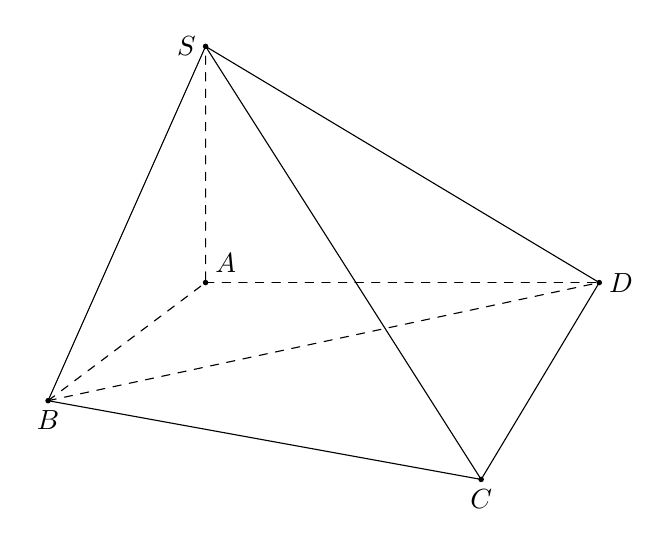
\begin{tikzpicture}[>=stealth, line join=round, line cap = round]
        \def\a{-1.5} \def\b{2} \def\c{3} \def\x{5}
\coordinate (S) at (0,\c);
\coordinate (A) at (0,0);
\coordinate (B) at (-\b,\a);
\coordinate (D) at (\x,0);
\coordinate (C) at ({\x -1.5},{\a - 1});
        \draw (S) node[left]{$S$} -- (B) node[below]{$B$} -- (C) node[below]{$C$} -- (D) node[right]{$D$} -- (S) -- (C);
        \draw[dashed] (A) node[above right]{$A$} -- (D);
        \draw[dashed] (B) -- (A) -- (S);
        \draw[dashed] (B) -- (D);
\fill (A)circle(1pt) 
(B)circle(1pt) 
(C)circle(1pt) 
(S)circle(1pt)
(D)circle(1pt); 
    \end{tikzpicture}
\end{center}
\choice
{\True $\dfrac{20\sqrt{273}}{819}$}
{$\dfrac{\sqrt{91}}{9}$}
{$\dfrac{3\sqrt{273}}{20}$}
{$\dfrac{9\sqrt{91}}{9}$}
\loigiai{
\begin{center}
    \begin{tikzpicture}[>=stealth, line join=round, line cap = round]
        \def\a{-1.5} \def\b{2} \def\c{3} \def\x{5}
\coordinate (S) at (0,\c);
\coordinate (A) at (0,0);
\coordinate (B) at (-\b,\a);
\coordinate (D) at (\x,0);
\coordinate (C) at ({\x -1.5},{\a - 1});
\coordinate (H) at ($(B)!0.4!(D)$);
        \draw (S) node[left]{$S$} -- (B) node[below]{$B$} -- (C) node[below]{$C$} -- (D) node[right]{$D$} -- (S) -- (C);
        \draw[dashed] (A) node[above left]{$A$} -- (D);
        \draw[dashed] (B) -- (A) -- (S);
        \draw[dashed] (B) -- (D);
        \draw[dashed] (A) -- (H) node[below]{$H$} -- (S);
\fill (A)circle(1pt) 
(B)circle(1pt) 
(C)circle(1pt) 
(S)circle(1pt)
(D)circle(1pt) 
(H)circle(1pt);
    \end{tikzpicture}
\end{center}
Có: $V_{S.ABCD}=\dfrac{1}{3}.SA.S_{ABCD}\Leftrightarrow 66\sqrt{3}=\dfrac{1}{3}.9.S_{ABCD}\Rightarrow{S_{ABCD}}=44\sqrt{3}$\\
Suy ra $\dfrac{1}{2}AB.AD+\dfrac{1}{2}BC.CD=44\sqrt{3}\Leftrightarrow 5AD+3CD=44$ . (1)\\
Áp dụng định lí Pitago trong 2 tam giác vuông $ABD;BCD$ , ta có:\\
$A{B^2}+A{D^2}=B{D^2}=B{C^2}+C{D^2}\Leftrightarrow C{D^2}-A{D^2}=48$ (2)\\
Từ (1) và (2) suy ra $\left[\begin{matrix}
AD=4\\
AD=\dfrac{47}{2}\\
\end{matrix}\right.$\\
$AD=\dfrac{47}{2}$ không thỏa mãn do từ (1) ta có: $AD<\dfrac{44}{5}\Rightarrow AD=4$ .\\
Trong tam giác $ABD$ , dựng $AH\perp BD$ lại có $SA\perp BD\Rightarrow BD\perp SH$ .\\
Vậy góc giữa $\left(SBD\right)$ và đáy là góc $\widehat{SHA}$ .\\
Dễ tính $BD=\sqrt{91},AH=\dfrac{AB.AD}{BD}=\dfrac{20\sqrt{273}}{91}$ , $\cot\widehat{SHA}=\dfrac{AH}{SA}=\dfrac{20\sqrt{273}}{819}$.}
\end{ex}

\begin{ex}[THPT Yên Khánh-Ninh Bình-2019]%[2H1K3-2]
Cho hình chóp $S.ABC$ có đáy $ABC$ là tam giác đều, $SA\perp\left(ABC\right)$ . Mặt phẳng $\left(SBC\right)$ cách $A$ một khoảng bằng $a$ và hợp với mặt phẳng $\left(ABC\right)$ góc $30^0$ . Thể tích của khối chóp $S.ABC$ bằng
\choice
{\True $\dfrac{8a^3}{9}$}
{$\dfrac{8a^3}{3}$}
{$\dfrac{\sqrt{3}{a^3}}{12}$}
{$\dfrac{4a^3}{9}$}
\loigiai{
\begin{center}
    \begin{tikzpicture}[>=stealth, line join=round, line cap = round]
        \def\a{-2.5} \def\b{3} \def\c{3} \def\x{5}
\coordinate (A) at (0,0);
\coordinate (S) at (0,\c);
\coordinate (B) at (\b,\a);
\coordinate (C) at (\x,0);
\coordinate (I) at ($(B)!0.5!(C)$);
\coordinate (H) at ($(S)!0.4!(I)$);
        \draw (S) node[left]{$S$} -- (A) node[left]{$A$} -- (B) node[below]{$B$} -- (C) node[right]{$C$} -- (S) -- (B);
        \draw[dashed] (A) -- (C);
        \draw[dashed] (A) -- (I) node[right]{$I$};
        \draw (I) circle(1pt) -- (S) circle(1pt);
        \draw[dashed] (A) -- (H) node[right]{$H$};
        \pic[draw,angle radius=3mm]{right angle=A--B--C};
        \pic[draw,angle radius=3mm]{right angle=C--A--S};
        \pic[draw,angle radius=3mm]{right angle=B--A--S};
        \pic[draw,angle radius=3mm]{right angle=A--H--I};
         \draw pic[draw,blue,fill=green!50,opacity=.5,angle radius=8mm,angle eccentricity=1.5,"$30^\circ$"] {angle = S--I--A};
\fill (A)circle(1pt) 
(B)circle(1pt) 
(C)circle(1pt) 
(S)circle(1pt)
(I)circle(1pt) 
(H)circle(1pt);
    \end{tikzpicture}
\end{center}

Gọi $I$ là trung điểm sủa $BC$ suy ra góc giữa mp $\left(SBC\right)$ và mp $\left(ABC\right)$ là $\widehat{SIA}=30^0$ .\\
$H$ là hình chiếu vuông góc của $A$ trên $SI$ suy ra $d\left(A,\left(SBC\right)\right)=AH=a$ .\\
Xét tam giác $AHI$ vuông tại $H$ suy ra $AI=\dfrac{AH}{\sin{30^0}}=2a$ .\\
Giả sử tam giác đều $ABC$ có cạnh bằng $x$ , mà $AI$ là đường cao suy ra $2a=x\dfrac{\sqrt{3}}{2}\Rightarrow x=\dfrac{4a}{\sqrt{3}}$ .\\
Diện tích tam giác đều $ABC$ là $S_{ABC}=\left(\dfrac{4a}{\sqrt{3}}\right)^2.\dfrac{\sqrt{3}}{4}=\dfrac{4a^2\sqrt{3}}{3}$ .\\
Xét tam giác $SAI$ vuông tại $A$ suy ra $SA=AI.\tan{30^0}=\dfrac{2a}{\sqrt{3}}$ .\\
Vậy $V_{S.ABC}=\dfrac{1}{3}.S_{ABC}.SA=\dfrac{1}{3}.\dfrac{4a^2\sqrt{3}}{3}.\dfrac{2a}{\sqrt{3}}=\dfrac{8a^3}{9}$ .}
\end{ex}


\begin{ex}%[2H1K3-2]
Cho khối chóp $ S.ABCD$ có đáy $ ABCD$ là hình vuông cạnh $ a$. Hai mặt phẳng $\left(SAB\right)$ và $\left(SAD\right)$ cùng vuông góc với đáy. Tính thể tích khối chóp $ S.ABCD$ biết rằng $ SC=a\sqrt{3}$.
\choice
{$V_{S.ABCD}=a^3$}
{\True $V_{S.ABCD}=\dfrac{a^3}{3}$}
{$V_{S.ABCD}=\dfrac{a^3\sqrt{3}}{3}$}
{$V_{S.ABCD}=\dfrac{a^3\sqrt{3}}{9}$}
\loigiai
{
\begin{center}
    \begin{tikzpicture}[>=stealth, line join=round, line cap = round]
        \def\a{-1.5} \def\b{2} \def\c{3} \def\x{5}
\coordinate (S) at (0,\c);
\coordinate (A) at (0,0);
\coordinate (B) at (-\b,\a);
\coordinate (D) at (\x,0);
\coordinate (C) at ($(B) + (D)$);
        \draw (S) node[left]{$S$} -- (B) node[below]{$B$} -- (C) node[below]{$C$} -- (D) node[right]{$D$} -- (S) -- (C);
        \draw[dashed] (A) node[above right]{$A$} -- (D);
        \draw[dashed] (B) -- (A) -- (S);
        \draw[dashed] (A) -- (C);
        \fill (A)circle(1pt) 
(B)circle(1pt) 
(C)circle(1pt) 
(S)circle(1pt)
(D)circle(1pt); 
    \end{tikzpicture}
\end{center}
Vì hai mặt phẳng $\left(SAB\right)$ và $\left(SAD\right)$ cùng vuông góc với đáy. Mà $\left(SAB\right)\cap\left(SAD\right)=SA$ nên $ SA\perp\left(ABCD\right)$.\\
Ta có: $ AC=a\sqrt{2}$; $SA=\sqrt{S{C^2}-A{C^2}}=\sqrt{\left(a\sqrt{3}\right)^2-\left(a\sqrt{2}\right)^2}=a$ .\\
Thể tích khối chóp $ S.ABCD$ là: $V_{S.ABCD}=\dfrac{1}{3}SA.S_{ABCD}=\dfrac{1}{3}a.a^2=\dfrac{a^3}{3}$.}
\end{ex}

\begin{ex}%[2H1K3-2]
Cho hình chóp $ S.ABC$có đáy là tam giác $ ABC$ vuông tại $ C$, $ AB=2a$, $ AC=a$ và $ SA$ vuông góc với mặt phẳng $\left(ABC\right)$. Biết góc giữa hai mặt phẳng $\left(SAB\right)$ và $\left(SBC\right)$ bằng $ 60^\circ $. Tính thể tích của khối chóp $ S.ABC$.
\choice
{$\dfrac{a^3\sqrt{2}}{6}$}
{\True $\dfrac{a^3\sqrt{6}}{12}$}
{$\dfrac{a^3\sqrt{6}}{4}$}
{$\dfrac{a^3\sqrt{2}}{2}$}
\loigiai
{\begin{center}
    \begin{tikzpicture}[>=stealth, line join=round, line cap = round]
        \def\a{-2.6} \def\b{2.5} \def\c{4} \def\x{6}
\coordinate (A) at (0,0);
\coordinate (S) at (0,\c);
\coordinate (C) at (\b,\a);
\coordinate (B) at (\x,0);
\coordinate (H) at ($(A)!0.4!(B)$);
\coordinate (K) at ($(S)!0.6!(B)$);
        \draw (S) node[left]{$S$} -- (A) node[left]{$A$} -- (C) node[below]{$C$} -- (B) node[right]{$B$} -- (S) -- (C) -- (K) node[right]{$K$};
        \draw[dashed] (A) -- (B);
        \draw[dashed] (C) -- (H) node[above left]{$H$} -- (K);

        \pic[draw,angle radius=3mm]{right angle=A--C--B};
        \pic[draw,angle radius=3mm]{right angle=C--H--B};
        \pic[draw,angle radius=3mm]{right angle=H--K--S};
        \pic[draw,angle radius=3mm]{right angle=C--K--B};
        \draw pic[draw,blue,fill=green!50,opacity=.5,angle radius=8mm,angle eccentricity=1.5,"$60^\circ$"] {angle = H--K--C};
\fill (A)circle(1pt) 
(B)circle(1pt) 
(C)circle(1pt) 
(S)circle(1pt)
(H)circle(1pt)
(K)circle(1pt);
    \end{tikzpicture}
\end{center}
Trong $\Delta ABC$kẻ $ CH\perp AB$$\Rightarrow CH\perp\left(SAB\right)$ $\Rightarrow CH\perp SB(1)$.\\
$ BC=\sqrt{A{B^2}-A{C^2}}=a\sqrt{3}$,\\
$ BH.BA=B{C^2}$,\\
$\Rightarrow BH=\dfrac{3a}{2}$, $ CH=\sqrt{B{C^2}-B{H^2}}=\dfrac{a\sqrt{3}}{2}$.\\
Trong $\Delta SAB$kẻ $ HK\perp SB$ $\Rightarrow CK\perp SB(2)$.\\
Từ $(1),(2)$ $\Rightarrow HK\perp SB$.\\
Góc giữa hai mặt phẳng $\left(SAB\right)$ và $\left(SBC\right)$ là $\widehat{CKH}=60^\circ $.\\
Trong vuông $\Delta CKH$ có $ HK=CH.\cot 60^\circ=\dfrac{a}{2}$, $BK=\sqrt{B{H^2}-H{K^2}}=a\sqrt{2}$ .\\
$\Delta SAB\backsim\Delta HKB\left(g.g\right)$ nên $\dfrac{SA}{HK}=\dfrac{AB}{BK}=\dfrac{2a}{a\sqrt{2}}$$\Rightarrow SA=\dfrac{a}{\sqrt{2}}$\\
Thể tích hình chóp $ S.ABC$ là $ V=\dfrac{1}{3}SA.S_{\Delta ABC}$$=\dfrac{1}{3}\dfrac{a}{\sqrt{2}}.\dfrac{1}{2}.a.\sqrt{3}.a=\dfrac{a^3\sqrt{6}}{12}$.}
\end{ex}


\begin{ex}%[2H1K3-2]
Cho khối chóp $ S.ABC$ có đáy $ ABC$ là tam giác cân tại $ A$ với $ BC=2a$, $\widehat{BAC}=120^\circ $, biết $ SA\perp (ABC)$ và mặt $ (SBC)$ hợp với đáy một góc $ 45^\circ $. Tính thể tích khối chóp $ S.ABC$.
\choice
{$\dfrac{a^3}{2}$}
{$a^3\sqrt{2}$}
{\True $\dfrac{a^3}{9}$}
{$\dfrac{a^3}{3}$}
\loigiai
{
\begin{center}
    \begin{tikzpicture}[>=stealth, line join=round, line cap = round]
        \def\a{-1.5} \def\b{1.5} \def\c{3} \def\x{5}
\coordinate (A) at (0,0);
\coordinate (S) at (0,\c);
\coordinate (B) at (\b,\a);
\coordinate (C) at (\x,0);
\coordinate (I) at ($(B)!0.5!(C)$);
        \draw (S) node[left]{$S$} -- (A) node[left]{$A$} -- (B) node[below]{$B$} -- (C) node[right]{$C$} -- (S) -- (B) circle(1pt);
        \draw[dashed] (A) circle(1pt) -- (C) circle(1pt);
        \draw[dashed] (A) -- (I) node[right]{$I$};
        \draw (I) circle(1pt) -- (S) circle(1pt);
        %\draw[dashed] (A)  -- (H) circle(1pt) node[right]{$H$};
        %\pic[draw,angle radius=3mm]{right angle=A--B--C};
        %\pic[draw,angle radius=3mm]{right angle=C--A--S};
        %\pic[draw,angle radius=3mm]{right angle=B--A--S};
        %\pic[draw,angle radius=3mm]{right angle=A--H--I};
        %\pic[draw,pos = 0.5,"$30^\circ$",angle radius=8mm]{angle=S--I--A};
    \end{tikzpicture}
\end{center}
Gọi $ I$ là trung điểm $ BC$.\\
+ Do $\Delta ABC$ cân tại $ A$ nên $ BC\perp AI$\\
+ Mặt khác do $SA\perp (ABC)\Rightarrow BC\perp SA$\\
Suy ra $ BC\perp SI$.\\
Do đó góc giữa $ (SBC)$ và đáy chính là góc $\widehat{SIA}=45^\circ $.\\
 Xét $\Delta AIB$ vuông tại $ I$ có $ IB=a$, $\widehat{IAB}=60^\circ $, suy ra $ IA=\dfrac{IB}{\tan 60^\circ}=\dfrac{a}{\sqrt{3}}$.\\
$\Delta SAI$ vuông tại $ A$ có $ IA=\dfrac{a}{\sqrt{3}}$, $\widehat{SIA}=45^\circ $ nên $\Delta SAI$ vuông cân tại $ A$, do đó $ SA=IA=\dfrac{a}{\sqrt{3}}$.\\
 Thể tích của khối chóp $ S.ABC$là $ V=\dfrac{1}{3}{S_{\Delta ABC}}.SA=\dfrac{1}{3}.\dfrac{1}{2}BC.AI.SA=\dfrac{a^3}{9}$.}
\end{ex}

\begin{ex}[Bạc Liêu – Ninh Bình]%[2H1K3-2]
Cho hình chóp $ S.ABCD$ có đáy $ ABCD$ là hình chữ nhật có $ AB=a$, $ AD=2a$; $ SA$ vuông góc với đáy, khoảng cách từ $ A$ đến $\left(SCD\right)$ bằng $\dfrac{a}{2}$. Tính thể tích của khối chóp theo $ a$.
\choice
{\True $\dfrac{4\sqrt{15}}{45}{a^3}$}
{$\dfrac{4\sqrt{15}}{15}{a^3}$}
{$\dfrac{2\sqrt{5}}{15}{a^3}$}
{$\dfrac{2\sqrt{5}}{45}{a^3}$}
\loigiai
{
\begin{center}
    \begin{tikzpicture}[>=stealth, line join=round, line cap = round]
        \def\a{-1.5} \def\b{2} \def\c{3.5} \def\x{5}
\coordinate (S) at (0,\c);
\coordinate (A) at (0,0);
\coordinate (B) at (-\b,\a);
\coordinate (D) at (\x,0);
\coordinate (C) at ($(B) + (D)$);
\coordinate (H) at ($(S)!0.4!(D)$);
        \draw (S) node[left]{$S$} -- (B) node[below]{$B$} -- (C) node[below]{$C$} -- (D) node[right]{$D$} -- (S) -- (C);
        \draw[dashed] (A) node[above left]{$A$} -- (D);
        \draw[dashed] (B) -- (A) -- (S);
        \draw[dashed] (A) -- (C);
        \draw[dashed] (A) -- (H) node[right]{$H$};
\fill (A)circle(1pt) 
(B)circle(1pt) 
(C)circle(1pt) 
(S)circle(1pt)
(H)circle(1pt)
(D)circle(1pt);
    \end{tikzpicture}
\end{center}
Gọi $ H$ là hình chiếu vuông góc của điểm $ A$ trên đường thẳng $ SD$. Ta có\\
$\left\{\begin{aligned}
& AH\perp SD\\ 
& AH\perp CD\\ 
\end{aligned}\right.$$\Rightarrow AH\perp\left(SCD\right)$$\Rightarrow AH=d\left(A,\left(SCD\right)\right)$. Suy ra $ AH=\dfrac{a}{2}$.\\
$\Delta SAD$ vuông tại $ A$ có đường cao $ AH$ nên\\
$\dfrac{1}{A{H^2}}=\dfrac{1}{S{A^2}}+\dfrac{1}{A{D^2}}$$\Leftrightarrow\dfrac{1}{S{A^2}}=\dfrac{1}{A{H^2}}-\dfrac{1}{A{D^2}}$$=\dfrac{15}{4a^2}$$\Rightarrow SA=\dfrac{2a\sqrt{15}}{15}$.\\
Vậy $ V=\dfrac{1}{3}AB.AD.SA$$=\dfrac{1}{3}a.2a.\dfrac{2a\sqrt{15}}{15}$$=\dfrac{4\sqrt{15}}{45}{a^3}$.}
\end{ex}


\begin{ex}[Cụm liên trường Hải Phòng-2019]%[2H1K3-2]
Cho hình chóp $ S.ABCD$ có đáy $ ABCD$ là hình vuông cạnh $ a$, $ SA$ vuông góc với đáy$ ABCD$, góc giữa hai mặt phẳng $\left(SBD\right)$ và $ ABCD$ bằng $60^0$. Gọi $ M\,,\,N$ lần lượt là trung điểm của $ SB\,,\,SC$. Tính thể tích khối chóp $ S.ADNM$.
\choice
{\True $V=\dfrac{a^3\sqrt{6}}{16}$}
{$V=\dfrac{a^3\sqrt{6}}{24}$}
{$V=\dfrac{3a^3\sqrt{6}}{16}$}
{$V=\dfrac{a^3\sqrt{6}}{8}$}
\loigiai{
\begin{center}
    \begin{tikzpicture}[>=stealth, line join=round, line cap = round]
        \def\a{-2.5} \def\b{2} \def\c{3.5} \def\x{5}
\coordinate (S) at (0,\c);
\coordinate (A) at (0,0);
\coordinate (B) at (-\b,\a);
\coordinate (D) at (\x,0);
\coordinate (C) at ($(B) + (D)$);
\coordinate (M) at ($(S)!0.5!(D)$);
\coordinate (N) at ($(S)!0.5!(C)$);
\coordinate (O) at (intersection of A--C and B--D);

        \draw (S) node[left]{$S$} -- (B) node[below]{$B$} -- (C) node[below]{$C$} -- (D) node[right]{$D$} -- (S) -- (C);
        \draw[dashed] (A) node[above left]{$A$} -- (D);
        \draw[dashed] (B) -- (A) -- (S);
        \draw[dashed] (A) -- (C);
        \draw[dashed] (B) -- (D);
        \draw[dashed] (A) -- (N);
        \draw[dashed] (A) -- (M) node[right]{$M$};
        \draw (M) -- (N) node[right]{$N$} -- (B);
        \draw[dashed] (S) -- (O) node[below]{$O$};

    \pic[draw,angle radius=3mm]{right angle=A--O--B};
    \pic[draw,angle radius=3mm]{right angle=D--O--S};
\fill (A)circle(1pt) 
(B)circle(1pt) 
(C)circle(1pt) 
(S)circle(1pt)
(D)circle(1pt)
(O)circle(1pt)
(M)circle(1pt)
(N)circle(1pt);
    \end{tikzpicture}
\end{center}
Gọi $ O=AC\cap BD$.\\
$ AO\perp BD\Rightarrow SO\perp BD$. Nên góc của $\left(SBD\right)$ và $ ABCD$ là góc $\widehat{SOA}=60^0$.\\
$V_{S.ADN}=\dfrac{1}{2}.V_{S.ADC}=\dfrac{1}{4}.V_{S.ABCD}$ và $V_{S.AMN}=\dfrac{1}{2}.\dfrac{1}{2}{V_{S.ABC}}=\dfrac{1}{8}{V_{S.ABCD}}$.\\
$\Rightarrow{V_{S.ADMN}}=V_{S.ADN}+V_{S.AMN}=\dfrac{3}{8}{V_{S.ABCD}}$.\\
$ SA=AO.\tan\widehat{SOA}=\dfrac{a\sqrt{2}}{2}\tan{60^0}=\dfrac{a\sqrt{6}}{2}$ $\Rightarrow{V_{S.ABCD}}=\dfrac{1}{3}{S_{ABCD}}.SA=\dfrac{a^3\sqrt{6}}{6}$.\\
$\Rightarrow{V_{S.ADMN}}=\dfrac{3}{8}.\dfrac{a^3\sqrt{6}}{6}=\dfrac{a^3\sqrt{6}}{16}$.}
\end{ex}

\begin{ex}[Chuyên Lê Quý Đôn Điện Biên 2019]%[2H1K3-2]
Cho khối chóp $ S.ABCD$ có đáy là hình vuông cạnh $ a$, $ SA$ vuông góc với đáy và khoảng cách từ $ C$ đến mặt phẳng $\left(SBD\right)$ bằng $\dfrac{a\sqrt{3}}{3}$. Tính thể tích $ V$ của khối chóp đã cho.
\choice
{$ V=\dfrac{a^3}{2}$}
{$ V=a^3$}
{\True $ V=\dfrac{a^3}{3}$}
{$ V=\dfrac{\sqrt{3}{a^3}}{9}$}
\loigiai
{\begin{center}
    \begin{tikzpicture}[>=stealth, line join=round, line cap = round]
        \def\a{-2.5} \def\b{2} \def\c{3.5} \def\x{6}
\coordinate (S) at (0,\c);
\coordinate (A) at (0,0);
\coordinate (B) at (-\b,\a);
\coordinate (D) at (\x,0);
\coordinate (C) at ($(B) + (D)$);
\coordinate (O) at (intersection of A--C and B--D);
\coordinate (H) at ($(S)!0.6!(O)$);
        \draw (S) node[left]{$S$} -- (B) node[below]{$B$} -- (C) node[below]{$C$} -- (D) node[right]{$D$} -- (S) -- (C);
        \draw[dashed] (A) node[above left]{$A$} -- (D);
        \draw[dashed] (B) -- (A) -- (S);
        \draw[dashed] (A) -- (C);
        \draw[dashed] (B) -- (D);
        \draw[dashed] (S) -- (O) node[below]{$O$};
        \draw[dashed] (A) -- (H) node[right]{$H$};
\fill (A)circle(1pt) 
(B)circle(1pt) 
(C)circle(1pt) 
(S)circle(1pt)
(D)circle(1pt)
(O)circle(1pt)
(H)circle(1pt);
    \end{tikzpicture}
\end{center}
Gọi $ O=AC\cap BD$, gọi $ H$ là hình chiếu của $ A$ lên $ SO$.\\
Vì $ O$ là trung điểm của $ AC$ nên $ d\left(C,\left(SBD\right)\right)=d\left(A,\left(SBD\right)\right)$\\
Ta có: $ BD\perp AC;\ BD\perp SA\\Rightarrow BD\perp\left(SAC\right)\Rightarrow\left(SBD\right)\perp\left(SAC\right);\ $\\
$ SO=\left(SAC\right)\cap\left(SBD\right)$\\
$ AH\perp SO\Rightarrow AH\perp\left(SBD\right)\Rightarrow AH=d\left(A,\left(SBD\right)\right)=d\left(C,\left(SBD\right)\right)=\dfrac{a\sqrt{3}}{3}$\\
Ta có: $ AO=\dfrac{a\sqrt{2}}{2}$.\\
Trong tam giác $ SAO:\dfrac{1}{A{H^2}}=\dfrac{1}{S{A^2}}+\dfrac{1}{A{O^2}}\Rightarrow SA=a$.\\
$V_{SABCD}=\dfrac{1}{3}.S_{ABCD}.SA=\dfrac{a^3}{3}$.}
\end{ex}



\begin{ex}[Bỉm Sơn-Thanh Hóa-2019]%[2H1K3-2]
Cho hình chóp S.ABCD có đáy là hình vuông cạnh a, SA vuông góc với mặt đáy, SD tạo với mặt phẳng $\left(SAB\right)$ một góc bằng $ 30^\circ $. Tính thể tích V của khối chóp S.ABCD.
\choice
{$ V=\sqrt{3}{a^3}$}
{\True $ V=\dfrac{\sqrt{3}{a^3}}{3}$}
{$ V=\dfrac{\sqrt{6}{a^3}}{18}$}
{$ V=\dfrac{\sqrt{6}{a^3}}{3}$}
\loigiai
{\begin{center}
    \begin{tikzpicture}[>=stealth, line join=round, line cap = round]
        \def\a{-1.5} \def\b{2} \def\c{3.5} \def\x{5}
\coordinate (S) at (0,\c);
\coordinate (A) at (0,0);
\coordinate (B) at (-\b,\a);
\coordinate (D) at (\x,0);
\coordinate (C) at ($(B) + (D)$);
        \draw (S) node[left]{$S$} -- (B) node[below]{$B$} -- (C) node[below]{$C$} -- (D) node[right]{$D$} -- (S) -- (C);
        \draw[dashed] (A) node[above left]{$A$} -- (D);
        \draw[dashed] (B) -- (A) -- (S);
    \fill (A)circle(1pt) 
(B)circle(1pt) 
(C)circle(1pt) 
(S)circle(1pt)
(D)circle(1pt);
    \end{tikzpicture}
\end{center}
Ta có hình chóp S.ABCD có đáy là hình vuông cạnh, SA vuông góc với mặt đáy nên $ DA\perp AB\,$và $ DA\perp SA\,$. Suy ra $ DA\perp\left(SAB\right)$. Vậy góc giữa SD và mặt phẳng $\left(SAB\right)$ là $\widehat{DSA}=30^\circ $.\\
Ta có $\,SA=AD.cot30^\circ=a\sqrt{3}$\\
$ V=\dfrac{1}{3}.SA.S_{ABCD}=\dfrac{1}{3}.a\sqrt{3}.a^2=\dfrac{\sqrt{3}}{3}{a^3}$.}
\end{ex}

\begin{ex}[Thpt Vĩnh Lộc-Thanh Hóa 2019]%[2H1K3-2]
Cho hình chóp $ S.ABCD$ có đáy $ ABCD$ là hình thoi, góc $ BAD$ bằng $120^0$,$ AB=a$. Hai mặt phẳng $\left(SAB\right)$ và $\left(SAD\right)$ cùng vuông góc với đáy. Góc giữa $\left(SBC\right)$ và mặt phẳng đáy là $60^0$. Tính thể tích $ V$ của chóp $ S.ABCD$.
\choice
{$ V=\dfrac{2a^3\sqrt{15}}{15}$}
{$ V=\dfrac{a^3}{12}$}
{\True $ V=\dfrac{a^3\sqrt{3}}{4}$}
{$ V=\dfrac{a^3\sqrt{13}}{12}$}
\loigiai
{\begin{center}
    \begin{tikzpicture}[>=stealth, line join=round, line cap = round]
        \def\a{-1.5} \def\b{2} \def\c{3.5} \def\x{5}
\coordinate (S) at (0,\c);
\coordinate (A) at (0,0);
\coordinate (B) at (-\b,\a);
\coordinate (D) at (\x,0);
\coordinate (C) at ($(B) + (D)$);
\coordinate (I) at ($(B)!0.55!(C)$);
        \draw (S) node[left]{$S$} -- (B) node[below]{$B$} -- (C) node[below]{$C$} -- (D) node[right]{$D$} -- (S) -- (C);
        \draw[dashed] (A) node[above left]{$A$} -- (D) node[pos=0.5,sloped,above]{$a$};
        \draw[dashed] (B) -- (A) -- (S);
        \draw[dashed] (A) -- (C);
        \draw[dashed] (A) -- (I) node[below]{$I$};
        \draw (S) -- (I);
\fill (A)circle(1pt) 
(B)circle(1pt) 
(C)circle(1pt) 
(S)circle(1pt)
(D)circle(1pt)
(I)circle(1pt);
    \end{tikzpicture}
\end{center}
Vì hai mặt phẳng $\left(SAB\right)$ và $\left(SAD\right)$ cùng vuông góc với đáy nên $ SA\perp mp\left(ABCD\right)$.\\
Ta có tam giác $ ABC$ đều cạnh $ a$, gọi $ I$ là trung điểm của $ BC$ khi đó:$ AI=\dfrac{a\sqrt{3}}{2}$\\
Và góc giữa $\left(SBC\right)$ và mặt phẳng đáy là $\widehat{SIA}=60^0$.\\
Xét tam giác $ SAI$ ta có:$\dfrac{SA}{AI}=\tan\left(\overset\frown{SIA}\right)\Rightarrow SA=AI\tan\left(60^0\right)\Rightarrow SA=\dfrac{3a}{2}$.\\
Ta có diện tích đáy $ ABCD$là:$S_{ABCD}=2S_{ABC}=2\left(\dfrac{1}{2}AI.BC\right)=\dfrac{a\sqrt{3}}{2}a=\dfrac{a^2\sqrt{3}}{2}$.\\
Thể tích của chóp $ S.ABCD$là: $V=\dfrac{1}{3}SA.S_{ABCD}=\dfrac{1}{3}.\dfrac{3a}{2}.\dfrac{a^2\sqrt{3}}{2}=\dfrac{a^3\sqrt{3}}{4}$.}
\end{ex}
\begin{dang}
	{Thể tích khối chóp đều }
\end{dang}

\begin{ex}%[2H1K3-2]%Câu 37
	(Chuyên Trần Phú Hải Phòng 2019) Cho khối chóp tứ giác đều $S.ABCD$ có cạnh đáy bằng $a$, góc giữa mặt bên và mặt đáy bằng $60^\circ$. Thể tích $V$ của khối chóp $S.ABCD$ bằng
	\choice
	{$V=\dfrac{a^3\sqrt{3}}{2}$}
	{$V=\dfrac{a^3\sqrt{2}}{2}$}
	{\True $V=\dfrac{a^3\sqrt{3}}{6}$}
	{$V=\dfrac{a^3\sqrt{2}}{6}$}
	\loigiai{
		\immini{
			Gọi $ O$ là tâm của đáy, gọi $M$ là trung điểm của $BC$.\\
			Ta có $\left\{\begin{aligned}
				& SO\perp BC\\ 
				& OM\perp BC\\ 
			\end{aligned}\right.$ nên $\left(SOM\right)\perp BC$, suy ra $\left[\left(SCD\right),\left(ABCD\right)\right]=\left(SM,OM\right)=\widehat{SMO}=60^\circ$.\\
			Có $OM=\dfrac{1}{2}BC=\dfrac{a}{2}$, $SO=OM\tan{60^\circ}=\dfrac{a\sqrt{3}}{2}$.\\
			Thể tích khối chóp $S.ABCD$ là\\
			$V_{S.ABCD}=\dfrac{1}{3}SO\cdot S_{ABCD}=\dfrac{1}{3}\cdot \dfrac{a\sqrt{3}}{2}\cdot a^2=\dfrac{a^3\sqrt{3}}{6}$.
		}{
			\begin{tikzpicture}[>=stealth,line join=round,line cap=round,font=\footnotesize,scale=.9]
				\path (0,0)coordinate (B) +(40:2)coordinate (A)+(0:4)coordinate (C) 
				(C)+(40:2)coordinate (D) ($(A)!.5!(C)$)coordinate (O)++(90:3.5)coordinate (S)
				($(D)!.5!(C)$)coordinate (M);
				\draw (S)--(B)--(C)--(S)--(M) (C)--(D)--(S);
				\draw[dashed] (B)--(D)--(A)--(O)--(M) (O)--(S) (B)--(A)--(S);
				\foreach \i/\j in {A/135,B/-135,C/-45,D/35,S/90,O/-95,M/-30}
				\fill[black] (\i) circle (1pt) (\i) node[shift={(\j:2.5mm)}]{$\i$};
			\end{tikzpicture}
		}
	}
\end{ex}

\begin{ex}%[2H1K3-2]%Câu 38
	(HSG Bắc Ninh 2019) Cho hình chóp tứ giác đều $S.ABCD$ có cạnh đáy bằng $a$, tâm của đáy là $O$. Gọi $M$ và $N$ lần lượt là trung điểm của $SA$ và $BC$. Biết góc giữa đường thẳng $MN$ và mặt phẳng $\left(ABCD\right)$ bằng $60^\circ$. Tính thể tích khối chóp $S.ABCD$.
	\choice
	{$\dfrac{a^3\sqrt{10}}{6}$}
	{$\dfrac{a^3\sqrt{30}}{2}$}
	{\True $\dfrac{a^3\sqrt{30}}{6}$}
	{$\dfrac{a^3\sqrt{10}}{3}$}
	\loigiai{
		\immini{
			Gọi $H$ là trung điểm $AO$. Khi đó góc giữa $MN$ và $\left(ABCD\right)$ là $\widehat{MNH}$.\\
			Ta có
			$ \begin{aligned}[t] 
				HN &=\sqrt{CN^2+CH^2-2CN\cdot CH\cdot \cos{45^\circ}} \\
				&= \dfrac{a\sqrt{10}}{4}.
			\end{aligned}$\\
			Suy ra $MH=HN\cdot \tan{60^\circ}=\dfrac{a\sqrt{10}}{4}\cdot \sqrt{3}=\dfrac{a\sqrt{30}}{4}$.\\
			Do đó $SO=2MH=\dfrac{a\sqrt{30}}{2}$.	
		}{
			\begin{tikzpicture}[>=stealth,line join=round,line cap=round,font=\footnotesize,scale=1]
				\path (0,0)coordinate (A) +(40:2)coordinate (D)+(0:4)coordinate (B) 
				(B)+(40:2)coordinate (C) ($(A)!.5!(C)$)coordinate (O)++(90:3.5)coordinate (S)
				($(S)!.5!(A)$)coordinate (M) ($(B)!.5!(C)$)coordinate (N) ($(A)!.5!(O)$)coordinate (H);
				\draw (B)--(S)--(A)--(B)--(C)--(S)--(M);
				\draw[dashed] (B)--(D)--(A)--(O) (O)--(S)--(D)--(C)--(O) (M)--(N)--(H)--(M);
				\foreach \i/\j in {A/-135,B/-45,C/0,D/35,S/90,O/-95,M/130,N/-35,H/-90}
				\fill[black] (\i) circle (1pt) (\i) node[shift={(\j:2.5mm)}]{$\i$};
			\end{tikzpicture}	
		}
	}
\end{ex}

\begin{ex}%[2H1K3-2]%Câu 39
	(Chuyên Lê Quý Đôn Quảng Trị 2019) Nếu một hình chóp tứ giác đều có cạnh đáy bằng $2$ và có diện tích xung quanh bằng $4\sqrt{3}$ thì có thể tích bằng
	\choice
	{\True $\dfrac{4\sqrt{2}}{3}$}
	{$4\sqrt{3}$}
	{$\dfrac{4\sqrt{3}}{3}$}
	{$4\sqrt{2}$}
	\loigiai{
		\immini{
			Xét hình chóp đều $S.ABCD$ như hình vẽ.\\
			Kẻ $OE\perp BC\Rightarrow E$ là trung điểm $BC$ và $BC\perp(SOE)$.\\
			Do đó $BC\perp SE$.\\
			Xét $\Delta SOE$ vuông tại $O$, ta có\\
			$SE^2=SO^2+OE^2 \Rightarrow SE=\sqrt{SO^2+1}$.\\
			Mặt khác
			$\begin{aligned}[t]
				&S_{xq}=4S_{\Delta SBC}\\ 
				&\Leftrightarrow 4\sqrt{3}=4\cdot \dfrac{1}{2}\cdot SE\cdot BC\\ 
				&\Leftrightarrow 4\sqrt{3}=2\cdot \sqrt{SO^2+1}\cdot 2\\ 
				&\Leftrightarrow SO=\sqrt{2}\;\left(x>0\right).
			\end{aligned}$\\
			$V_{S.ABCD}=\dfrac{1}{3}\cdot SO\cdot S_{ABCD}=\dfrac{1}{3}\cdot \sqrt{2}\cdot 2^2=\dfrac{4\sqrt{2}}{3}$ (đvtt).	
		}{
			\begin{tikzpicture}[>=stealth,line join=round,line cap=round,font=\footnotesize,scale=1]
				\path (0,0)coordinate (D) +(40:2)coordinate (A)+(0:4)coordinate (C) 
				(C)+(40:2)coordinate (B) ($(A)!.5!(C)$)coordinate (O)++(90:4)coordinate (S)
				($(B)!.5!(C)$)coordinate (E);
				\draw (B)--(S)--(E) (B)--(C)--(D)--(S)--(C);
				\draw[dashed] (A)--(B)--(D)--(A)--(O)--(E) (C)--(O)--(S)--(A);
				\foreach \i/\j in {A/135,B/35,C/-45,D/-135,S/90,O/-95,E/-30}
				\fill[black] (\i) circle (1pt) (\i) node[shift={(\j:2.5mm)}]{$\i$};
			\end{tikzpicture}	
		}
	}
\end{ex}

\begin{ex}%[2H1K3-2]%Câu 40
	Cho hình chóp đều $S.ABC$ có $SA=a$. Gọi $D$, $E$ lần lượt là trung điểm của $SA$, $SC$. Tính thể tích khối chóp $S.ABC$ theo $a$, biết $BD$ vuông góc với $AE$.
	\choice
	{\True $\dfrac{a^3\sqrt{21}}{54}$}
	{$\dfrac{a^3\sqrt{3}}{12}$}
	{$\dfrac{a^3\sqrt{7}}{27}$}
	{$\dfrac{a^3\sqrt{21}}{27}$}
	\loigiai{
		\immini{
			Gọi $F$ là trung điểm $SE$ $\Rightarrow BD\perp DF$; gọi $AB=x$.\\
			Ta có\\
			$\begin{aligned}[t] 
				BE^2 &=BD^2=AE^2 = \dfrac{2AS^2+2AC^2-SC^2}{4}\\
				&= \dfrac{2a^2+2x^2-a^2}{4}=\dfrac{a^2+2x^2}{4}.
			\end{aligned}$
			
			$\begin{aligned}[t] 
				BF^2 &= \dfrac{2BS^2+2BE^2-SE^2}{4}=\dfrac{2a^2+\dfrac{a^2+2x^2}{2}-\dfrac{a^2}{4}}{4}\\
				&= \dfrac{9a^2+4x^2}{16}.
			\end{aligned}$
			$\begin{aligned}[t]
				& BF^2=BD^2+DF^2\Leftrightarrow BF^2=\dfrac{5BD^2}{4}.\\ 
				&\Leftrightarrow\dfrac{9a^2+4x^2}{16}=\dfrac{5}{4}\cdot \dfrac{a^2+2x^2}{4}\Leftrightarrow 9a^2+4x^2=5a^2+10x^2\Leftrightarrow 4a^2=6x^2\Rightarrow x=a\sqrt{\dfrac{2}{3}}.\\ 
			\end{aligned}$
		}{
			\begin{tikzpicture}[>=stealth,line join=round,line cap=round,font=\footnotesize,scale=1]
				\path (0,0)coordinate (A) (0:5)coordinate (C) (-40:2.5)coordinate (B)
				($(A)!.5!(B)$)coordinate (M) ($(B)!.5!(C)$)coordinate (N) 
				(intersection of A--N and C--M)coordinate (H) ++(90:4)coordinate (S)
				($(S)!.5!(A)$)coordinate (D) ($(S)!.5!(C)$)coordinate (E) ($(S)!.5!(E)$)coordinate (F);
				\draw (F)--(B)--(S)--(A)--(B)--(C)--(S) (D)--(B)--(E);
				\draw[dashed] (E)--(A)--(C)--(M) (D)--(F) (A)--(N) (S)--(H);
				\foreach \i/\j in {A/180,B/-90,C/0,S/90,D/135,E/45,F/50,H/50}
				\fill[black] (\i) circle (1pt) (\i) node[shift={(\j:2.5mm)}]{$\i$};
			\end{tikzpicture}
		}
		\noindent Gọi $H$ là hình chiếu của $S$ lên $\left(ABC\right)$ khi đó $H$ là tâm đường tròn ngoại tiếp $\Delta ABC$.\\
		Suy ra $SH=\sqrt{SA^2-AH^2}=\sqrt{a^2-\left(\dfrac{2}{3}\cdot \dfrac{x\sqrt{3}}{2}\right)^2}=\dfrac{a\sqrt{7}}{3}$.\\
		Tam giác $ABC$ đều có cạnh là $x\Rightarrow S_{\Delta ABC}=\dfrac{x^2\sqrt{3}}{4}=\dfrac{a^2\sqrt{3}}{6}$.\\
		Vậy $V_{S.ABC}=\dfrac{1}{3}SH\cdot S_{\Delta ABC}=\dfrac{1}{3}\cdot \dfrac{a\sqrt{7}}{3}\cdot \dfrac{a^2\sqrt{3}}{6}=\dfrac{a^3\sqrt{21}}{54}$.\\
		Hoặc sử dụng công thức tính thể tích chóp tam giác $ABC$ đều có cạnh bên bằng $a$, cạnh đáy bằng $x$.\\
		$V_{S.ABC}=\dfrac{x^2\cdot \sqrt{3a^2-x^2}}{12}=\dfrac{\dfrac{2a}{3}^2\sqrt{3a^2-\dfrac{2a}{3}^2}}{12}=\dfrac{a^3\sqrt{21}}{54}$.
	}
\end{ex}

\begin{ex}%[2H1K3-2]%Câu 41
	Cho hình chóp đều $S.ABCD$ có cạnh $AB=a$, góc giữa đường thẳng $SA$ và mặt phẳng $\left(ABC\right)$ bằng $45^\circ $. Thể tích khối chóp $S.ABCD$ là
	\choice
	{$\dfrac{a^3}{3}$}
	{\True $\dfrac{a^3\sqrt{2}}{6}$}
	{$\dfrac{a^3}{6}$}
	{$\dfrac{a^3\sqrt{2}}{3}$}
	\loigiai{
		\immini{
			Vì $S.ABCD$ là hình chóp đều nên đáy $ABCD$ là hình vuông và chân đường cao $H$ trùng với tâm của hình vuông $ ABCD$.\\
			Diện tích đáy của khối chóp $S.ABCD$ là $S_{ABCD}=a^2$.\\
			Nhận thấy $HA$ là hình chiếu vuông góc của $SA$ trên $\left(ABC\right)$. Vì thế $\left(SA,\left(ABC\right)\right)=\left(SA,HA\right)=\widehat{SAH}$.\\
			Suy ra $\widehat{SAH}=45^\circ $.\\
			Xét tam giác $ABC$ vuông tại $B$, ta có\\ 
			$AC=\sqrt{AB^2+BC^2}=a\sqrt{2}$. Suy ra $HA=\dfrac{a\sqrt{2}}{2}$.\\
			Tam giác $SHA$ vuông tại $H$ và có $\widehat{SAH}=45^\circ $ nên là tam giác vuông cân tại $H$. Suy ra $SH=HA=\dfrac{a\sqrt{2}}{2}$.	
		}{
			\begin{tikzpicture}[>=stealth,line join=round,line cap=round,font=\footnotesize,scale=1]
				\path (0,0)coordinate (B) +(40:2)coordinate (A)+(0:4)coordinate (C) 
				(C)+(40:2)coordinate (D) ($(A)!.5!(C)$)coordinate (H)++(90:4)coordinate (S);
				\draw (C)--(S)--(B)--(C)--(D)--(S);
				\draw[dashed] (S)--(A)--(B)--(D)--(A)--(C) (O)--(S);
				\draw pic["$45^\circ$"{scale=.8},draw,angle radius=10,angle eccentricity=1.75] {angle = C--A--S};
				\foreach \i/\j in {A/135,B/-135,C/-45,D/35,S/90,H/-95}
				\fill[black] (\i) circle (1pt) (\i) node[shift={(\j:2.5mm)}]{$\i$};
			\end{tikzpicture}	
		}
		\noindent Thể tích khối chóp $S.ABCD$ là: $V=\dfrac{1}{3}\cdot S_{ABCD}\cdot SH=\dfrac{1}{3}\cdot a^2\cdot\dfrac{a\sqrt{2}}{2}=\dfrac{a^3\sqrt{2}}{6}$.
	}
\end{ex}

\begin{ex}%[2H1K3-2]%Câu 42
	(HKI-NKHCM 2019) Cho hình chóp tứ giác đều $S.ABCD$ độ dài cạnh đáy là $a$. Biết rằng mặt phẳng $(P)$ qua $A$ và vuông góc với $SC$, cắt cạnh $SB$ tại $B'$ với $\dfrac{SB'}{SB}=\dfrac{2}{3}$. Tính thể tích của khối chóp $S.ABCD$
	\choice
	{\True $\dfrac{a^3\sqrt{6}}{6}$}
	{$\dfrac{a^3\sqrt{6}}{4}$}
	{$\dfrac{a^3\sqrt{6}}{2}$}
	{$\dfrac{a^3\sqrt{6}}{3}$}
	\loigiai{
		\immini{
			Ta có $\left.\begin{aligned}
				& BD\perp AC\\ 
				& BD\perp SO\\ 
			\end{aligned}\right\}\Rightarrow BD\perp\left(SAC\right)\Rightarrow BD\perp SC$.\\
			Mà $(P)\perp SC\Rightarrow(P)\parallel BD$.\\
			Trong $\left(SAC\right)$, gọi $G=AC'\cap SO$.\\
			Suy ra $GB'\parallel BD\Rightarrow\dfrac{SG}{SO}=\dfrac{SB'}{SB}=\dfrac{2}{3}$.\\
			Suy ra $G$ là trọng tâm $\Delta SAC\Rightarrow C'$ là trung điểm $SC$.\\
			Nên $\Delta SAC$ là tam giác đều cạnh $AC=a\sqrt{2}$.\\
			Suy ra $SO=a\sqrt{2}\cdot \dfrac{\sqrt{3}}{2}=a\dfrac{\sqrt{6}}{2}$\\
			$\Rightarrow{V_{SABCD}}=\dfrac{1}{3}{S_{ABCD}}\cdot SO=\dfrac{1}{3}{a^2}\cdot \dfrac{a\sqrt{6}}{2}=\dfrac{a^3\sqrt{6}}{6}$.	
		}{
			\begin{tikzpicture}[>=stealth,line join=round,line cap=round,font=\footnotesize,scale=1]
				\path (0,0)coordinate (A) +(40:2)coordinate (D)+(0:4)coordinate (B) 
				(B)+(40:2)coordinate (C) ($(A)!.5!(C)$)coordinate (O)++(90:4)coordinate (S)
				($(S)!2/3!(O)$)coordinate (G) ($(S)!2/3!(D)$)coordinate (D')
				($(S)!2/3!(B)$)coordinate (B') (intersection of A--G and S--C)coordinate (C');
				\draw (B)--(S)--(A)--(B)--(C)--(S);
				\draw[dashed] (B)--(D)--(A)--(C)--(D)--(S)--(O) (B')--(D') (A)--(C');
				\foreach \i/\j in {A/-160,B/-40,C/15,D/160,B'/0,C'/30,D'/180,S/90,G/0,O/-90}
				\fill[black] (\i) circle (1pt) ($(\i)+(\j:2.5mm)$)node{$\i$};
			\end{tikzpicture}	
		}
	}
\end{ex}

\begin{ex}%[2H1K3-2]%Câu 43
	(Sở Quảng Trị 2019) Cho một hình chóp tứ giác đều có cạnh đáy bằng $2a$ và cạnh bên tạo với mặt phẳng đáy một góc $45^\circ $. Thể tích của khối chóp đó là
	\choice
	{\True $\dfrac{4a^3\sqrt{2}}{3}$}
	{$\dfrac{a^3\sqrt{2}}{8}$}
	{$\dfrac{a^3\sqrt{2}}{6}$}
	{$2a^3\sqrt{2}$}
	\loigiai{
		\immini{
			Dựng hình chóp tứ giác đều $S.ABCD$ thỏa mãn các điều kiện đề bài với $O=AC\cap BD$.\\
			Theo giả thiết ta có $AB=2a$, $SA$ tạo với mặt phẳng $\left(ABCD\right)$ một góc $45^\circ $ suy ra $\widehat{SAO}=45^\circ $.\\
			$ABCD$ là hình vuông cạnh $2a$ nên tính được\\
			$AC=2\sqrt{2}a\Rightarrow OA=a\sqrt{2}$.\\
			Tam giác $SOA$ vuông cân tại $O$ vì có $SO\perp OA$, $\widehat{SAO}=~45^\circ $ suy ra $SO=OA=a\sqrt{2}$.\\
			Vậy thể tích khối chóp là\\ $V=\dfrac{1}{3}{S_{ABCD}}\cdot SO=\dfrac{1}{3}4a^2\cdot a\sqrt{2}=\dfrac{4a^3\sqrt{2}}{3}$.	
		}{
			\begin{tikzpicture}[>=stealth,line join=round,line cap=round,font=\footnotesize,scale=1]
				\path (0,0)coordinate (B) +(40:2)coordinate (A)+(0:4)coordinate (C) 
				(C)+(40:2)coordinate (D) ($(A)!.5!(C)$)coordinate (O)++(90:4)coordinate (S);
				\draw (S)--(B)--(C)--(S) (C)--(D)--(S);
				\draw[dashed] (B)--(D)--(A)--(C) (O)--(S)--(A)--(B);
				\draw pic["$45^\circ$"{scale=.8},draw,angle radius=10,angle eccentricity=1.75] {angle = C--A--S};
				\foreach \i/\j in {A/135,B/-135,C/-45,D/35,S/90,O/-95}
				\fill[black] (\i) circle (1pt) (\i) node[shift={(\j:2.5mm)}]{$\i$};
			\end{tikzpicture}	
		}
	}
\end{ex}

\begin{ex}%[2H1K3-2]%Câu 44
	(THPT Trần Phú 2019) Cho hình chóp tứ giác đều $S.ABCD$ có cạnh đáy bằng $2a\sqrt{3}$, khoảng cách giữa hai đường thẳng $SA$ và $CD$ bằng $3a$. Thể tích khối chóp đã cho bằng:
	\choice
	{$a^3\sqrt{3}$}
	{$6a^3\sqrt{3}$}
	{\True $12a^3$}
	{$\dfrac{8a^3\sqrt{3}}{3}$}
	\loigiai{
		\immini{
			Gọi $O=AC\cap BD$.\\
			Ta có $\left\{\begin{aligned}
				& CD \parallel AB\\ 
				& AB\subset (SAB)
			\end{aligned}\right.$
			$\Rightarrow d(CD,SA)=d\left(CD,(SAB)\right)$\\
			$=d\left(D,(SAB)\right)=2d(O,(SAB))$.\\
			Kẻ $\left\{\begin{aligned}
				& OK\perp AB\\ 
				& OH\perp SK\\ 
			\end{aligned}\right.\Rightarrow OH\perp(SAB)$\\
			$\Rightarrow OH=d\left(O,\left(SAB\right)\right)=\dfrac{3a}{2}$.\\
			Xét $\Delta SOK \colon\dfrac{1}{OH^2}=\dfrac{1}{SO^2}+\dfrac{1}{OK^2}\Leftrightarrow SO=3a$.	
		}{
			\begin{tikzpicture}[>=stealth,line join=round,line cap=round,font=\footnotesize,xscale=.8]
				\path (0,0)coordinate (D) +(30:2.5)coordinate (A)+(0:4)coordinate (C) 
				(C)+(30:2.5)coordinate (B) ($(A)!.5!(C)$)coordinate (O)++(90:3.5)coordinate (S)
				($(A)!.5!(B)$)coordinate (K) ($(S)!.7!(K)$)coordinate (H);
				\draw (S)--(B)--(C)--(D)--(S)--(C);
				\draw[dashed] (S)--(A)--(B)--(D)--(A)--(O)--(K) (C)--(O)--(S)--(K) (O)--(H);
				\foreach \i/\j/\k in {S/O/K,O/K/B,O/H/K}{
					\draw[cyan] ($(\j)!6pt!(\i)$)--($(\j)!6pt!(\k)-(\j)+(\j)!6pt!(\i)$)--($(\j)!6pt!(\k)$);};
				\foreach \i/\j in {A/135,B/35,C/-45,D/-135,S/90,O/-95,K/50,H/50}
				\fill[black] (\i) circle (1pt) (\i) node[shift={(\j:2.5mm)}]{$\i$};
			\end{tikzpicture}	
		}
		\noindent Vậy thể tích khối chóp $S.ABCD\colon V=\dfrac{1}{3}{S_{ABCD}}\cdot SO=12a^3$.
	}
\end{ex}

\begin{ex}%[2H1K3-2]%Câu 45
	(Kiểm tra năng lực-ĐH-Quốc Tế 2019) Cho hình chóp tam giác đều $S.ABC$, cạnh $AB=a$ và cạnh bên hợp với đáy một góc $45^\circ $. Thể tích $V$ của khối chóp là
	\choice
	{\True $V=\dfrac{a^3}{12}$}
	{$V=\dfrac{a^3}{6}$}
	{$V=\dfrac{a^3}{3}$}
	{$V=\dfrac{a^3}{4}$}
	\loigiai{
		\immini{
			Gọi $O$ là tâm đường tròn ngoại tiếp tam giác $ABC$.\\
			Vì $S.ABC$ là hình chóp tam giác đều nên $SO\perp\left(ABC\right)$.\\
			Do $S.ABC$ là hình chóp tam giác đều nên các cạnh bên đều tạo với mặt đáy các góc bằng nhau.\\
			Góc giữa cạnh $SC$ với đáy là góc giữa hai đường thẳng $SC$ và $OC$ hay chính là góc $\widehat{SCO}$.\\
			Theo bài ra ta có $\widehat{SCO}=45^\circ \Rightarrow\Delta SOC$ vuông cân tại $O$.\\
			Tam giác $ABC$ đều cạnh $a$ nên $ CO=SO=\dfrac{2}{3}\cdot \dfrac{a\sqrt{3}}{2}=\dfrac{a\sqrt{3}}{3}$.\\
			Diện tích đáy: $S_{ABC}=\dfrac{a^2\sqrt{3}}{4}$.\\
			Thể tích của khối chóp $V=\dfrac{1}{3}{S_{ABC}}\cdot SO=\dfrac{1}{3}\dfrac{a^2\sqrt{3}}{4}\cdot \dfrac{a\sqrt{3}}{3}=\dfrac{a^3}{12}$.	
		}{
			\begin{tikzpicture}[>=stealth,line join=round,line cap=round,font=\footnotesize,scale=1]
				\path (0,0)coordinate (A) +(0:4)coordinate (C) 
				+(-35:4)coordinate (B) (barycentric cs:A=1,B=1,C=1) coordinate (O) 
				++(90:3.5)coordinate (S) ($(A)!1/2!(B)$)coordinate (I) ($(A)!1/2!(C)$)coordinate (K);
				\draw (B)--(S)--(A)--(B)--(C)--(S);
				\draw[dashed] (A)--(C) (B)--(K) (I)--(C) (S)--(O);
				\foreach \i/\j/\k in {S/O/C}{
					\draw[cyan] ($(\j)!6pt!(\i)$)--($(\j)!6pt!(\k)-(\j)+(\j)!6pt!(\i)$)--($(\j)!6pt!(\k)$);};
				\foreach \i/\j in {A/180,B/-90,C/0,S/90,O/-110,I/-135}
				\fill[black] (\i) circle (1pt) (\i) node[shift={(\j:2.5mm)}]{$\i$};
			\end{tikzpicture}	
		}
	}
\end{ex}

\begin{ex}%[2H1K3-2]%Câu 46
	Cho khối chóp tứ giác đều có tất cả các cạnh bằng $2a$. Thể tích của khối chóp đã cho bằng:
	\choice
	{$\dfrac{2\sqrt{2}{a^3}}{3}$}
	{$\dfrac{8a^3}{3}$}
	{$\dfrac{8\sqrt{2}{a^3}}{3}$}
	{\True $\dfrac{4\sqrt{2}{a^3}}{3}$}
	\loigiai{
		\immini{
			Gọi $O$ là tâm của hình vuông $ABCD$, ta có $SO\perp\left(ABCD\right)$.\\
			Xét tam giác $SOA$ vuông tại $O$ có\\
			$SA=2a$, $AO=\dfrac{1}{2}AC=\dfrac{1}{2}\cdot 2a\sqrt{2}=a\sqrt{2}$.\\
			Suy ra $SO=\sqrt{SA^2-AO^2}=\sqrt{\left(2a\right)^2-\left(a\sqrt{2}\right)^2}=a\sqrt{2}$.\\
			Vậy $V_{S.ABCD}=\dfrac{1}{3}\cdot SO\cdot S_{ABCD}=\dfrac{1}{3}\cdot a\sqrt{2}\cdot \left(2a\right)^2=\dfrac{4a^3\sqrt{2}}{3}$.	
		}{
			\begin{tikzpicture}[>=stealth,line join=round,line cap=round,font=\footnotesize,scale=.8]
				\path (0,0)coordinate (B) +(40:2)coordinate (A)+(0:4)coordinate (C) 
				(C)+(40:2)coordinate (D) ($(A)!.5!(C)$)coordinate (O)++(90:3.5)coordinate (S);
				\draw (B)--(C)--(S) (C)--(D)--(S)--(B);
				\draw[dashed] (A)--(B)--(D)--(A)--(C) (O)--(S)--(A);
				\foreach \i/\j in {A/135,B/-135,C/-45,D/0,S/90,O/-95}
				\fill[black] (\i) circle (1pt) (\i) node[shift={(\j:2.5mm)}]{$\i$};
			\end{tikzpicture}	
		}
	}
\end{ex}

\begin{ex}%[2H1K3-2]%Câu 47
	(Đề minh họa 2022) Cho khối chóp đều $S.ABCD$ có $AC=4a$, hai mặt phẳng $(SAB)$ và $\left(SCD\right)$ vuông góc với nhau. Thể tích của khối chóp đã cho bằng.
	\choice
	{$\dfrac{16\sqrt{2}}{3}{a^3}$}
	{\True $\dfrac{8\sqrt{2}}{3}{a^3}$}
	{$16a^3$}
	{$\dfrac{16}{3}{a^3}$}
	\loigiai{
		\immini{
			Gọi $O$ là giao điểm của $AC$ và $BD$.\\
			Gọi $I$, $J$ lần lượt là trung điểm của cạnh $CD$ và $AB$.\\
			Vì $S.ABCD$ đều nên $SO\perp\left(ABCD\right)$.\\
			Ta có $\left\{\begin{aligned}
				& S\in\left(SAB\right)\cap\left(SBC\right)\\ 
				& AB\parallel CD.
			\end{aligned}\right.$\\
			Suy ra giao tuyến của hai mặt phẳng $\left(SAB\right)$ và $\left(SCD\right)$ là đường thẳng $ d$ đi qua $S$ và song song với $ AB,CD$.\\
			Hơn nữa, tam giác $SCD$ là tam giác cân tại $S$ có $SI$ là đường trung tuyến đồng thời là đường cao nên $SI\perp d$.\\
			Ta có $\left\{\begin{aligned}
				&(SAB)\perp (SCD)\\ 
				&(SAB)\cap (SCD)=d\\ 
				& SI\subset (SCD), \;SI\perp d\\ 
			\end{aligned}\right.\Rightarrow SI\perp\left(SAB\right)$.	
		}{
			\begin{tikzpicture}[>=stealth,line join=round,line cap=round,font=\footnotesize,scale=1]
				\path (0,0)coordinate (B) +(40:2)coordinate (A)+(0:4)coordinate (C) 
				(C)+(40:2)coordinate (D) ($(A)!.5!(C)$)coordinate (O)++(90:4)coordinate (S)
				($(C)!.5!(D)$)coordinate (I) ($(A)!.5!(B)$)coordinate (J);
				\draw[shorten >=-1.5cm,shorten <=-1cm] (S)--($(S)+(B)-(A)$) node[above, pos=1.2]{$d$};
				\draw (B)--(C)--(S) (C)--(D)--(S)--(B);
				\draw[dashed] (A)--(B)--(D)--(A)--(C) (O)--(S) (A)--(S)--(J)--(I);
				\foreach \i/\j in {A/135,B/-135,C/-45,D/0,S/90,O/-95,I/-45,J/-90}
				\fill[black] (\i) circle (1pt) (\i) node[shift={(\j:2.5mm)}]{$\i$};
			\end{tikzpicture}	
		}
		\noindent Mà $SJ\subset (SAB)$ nên $SI\perp SJ$.\\
		Dễ thấy $\Delta SOI=\Delta SOJ$ (c.g.c).\\
		Suy ra $SJ=SI$. Như vậy tam giác $SIJ$ vuông cân tại $S$.\\
		Ta có $AC=4a\Rightarrow AB=BC=IJ=\dfrac{AC}{\sqrt{2}}=2a\sqrt{2}$.\\
		Xét tam giác $SIJ$ vuông cân tại $S$, có\\
		$\left\{\begin{aligned}
			& SI=SJ=\dfrac{IJ}{\sqrt{2}}=\dfrac{2a\sqrt{2}}{\sqrt{2}}=2a\\ 
			& SO\cdot IJ=SJ\cdot SI\Leftrightarrow SO\cdot 2a\sqrt{2}=2a\cdot 2a\Rightarrow SO=a\sqrt{2}.
		\end{aligned}\right.$\\
		Thể tích khối chóp đều $S.ABCD$: $V_{S.ABCD}=\dfrac{1}{3}SO\cdot S_{ABCD}=\dfrac{1}{3}a\sqrt{2}\cdot \left(2a\sqrt{2}\right)^2=\dfrac{8\sqrt{2}}{3}{a^3}$.
	}
\end{ex}
\begin{ex}%[2H1K3-2]%Câu 48
	(Đề Minh Họa 2017) Cho tứ diện $ABCD$ có các cạnh $AB$, $AC$ và $AD$ đôi một vuông góc với nhau; $AB=6a$, $AC=7a$ và $AD=4a$. Gọi $ M$, $N$, $P$ tương ứng là trung điểm các cạnh $BC$, $CD$, $DB$. Tính thể tích $V$ của tứ diện $AMNP$.
	\choice
	{\True $V=7a^3$}
	{$V=14a^3$}
	{$V=\dfrac{28}{3}{a^3}$}
	{$V=\dfrac{7}{2}{a^3}$}
	\loigiai{
		\immini{
			Ta có $V_{ABCD}=\dfrac{1}{3}AB\cdot \dfrac{1}{2}AD\cdot AC=\dfrac{1}{6}6a\cdot 7a\cdot 4a=28a^3$.\\
			Ta nhận thấy $S_{MNP}=\dfrac{1}{2}{S_{MNPD}}=\dfrac{1}{4}{S_{BCD}}$.\\
			Suy ra ${V_{AMNP}}=\dfrac{1}{4}{V_{ABCD}}=7a^3$.	
		}{
			\begin{tikzpicture}[>=stealth,line join=round,line cap=round,font=\footnotesize,scale=.8]
				\path (0,0)coordinate (A) (0:4)coordinate (B) (-135:2)coordinate (C) 
				(90:3.5)coordinate (D) ($(B)!.5!(C)$)coordinate (M) ($(D)!.5!(C)$)coordinate (N)
				($(B)!.5!(D)$)coordinate (P);
				\draw (M)--(N)--(P)--(M)--(B)--(D)--(C)--(M);
				\draw[dashed] (M)--(A)--(N) (C)--(A)--(P) (B)--(A)--(D);
				\foreach \i/\j in {A/-85,B/0,C/-135,D/90,M/-80,N/180,P/45}
				\fill[black] (\i) circle (1pt) (\i) node[shift={(\j:2.5mm)}]{$\i$};
			\end{tikzpicture}	
		}
	}
\end{ex}

\begin{ex}%[2H1K3-2]
	(Chuyên Hùng Vương-Phú Thọ 2020) Cho hình chóp $S.ABCD$ có đáy $ABC$ là tam giác vuông cân đỉnh $A$, $AB=a\sqrt{2}$ Gọi $I$ là trung điểm của $BC$, hình chiếu vuông góc của đỉnh $S$ lên mặt phẳng $\left(ABC\right)$ là điểm $H$ thỏa mãn $\overrightarrow{IA}=-2\overrightarrow{IH}$, góc giữa $SC$ và mặt phẳng $\left(ABC\right)$ bằng $60^\circ $. Thể tích khối chóp $S.ABC$ bằng
	\choice
	{$\dfrac{a^3\sqrt{5}}{2}$}
	{$\dfrac{a^3\sqrt{5}}{6}$}
	{\True $\dfrac{a^3\sqrt{15}}{6}$}
	{$\dfrac{a^3\sqrt{15}}{12}$}
	\loigiai{
		\immini{
			$S_{ABC}=\dfrac{1}{2}AB\cdot AC=\dfrac{1}{2}\cdot a\sqrt{2}\cdot a\sqrt{2}=a^2$.\\
			$BC=2a$, $IA=a$, $IH=\dfrac{a}{2}$.\\
			Tam giác $HIC$ vuông tại $I$ ta có\\ $HC^2=HI^2+IC^2=\dfrac{a^2}{4}+a^2=\dfrac{5a^2}{4}\Rightarrow HC=\dfrac{a\sqrt{5}}{2}$.\\
			$\tan\widehat{SCH}=\dfrac{SH}{HC}\Leftrightarrow SH=HC\cdot \tan\widehat{SCH}=\dfrac{a\sqrt{5}}{2}\cdot \sqrt{3}=\dfrac{a\sqrt{15}}{2}$.\\
			Vậy $V_{S.ABC}=\dfrac{1}{3}\cdot SH\cdot S_{ABC}=\dfrac{1}{3}\cdot \dfrac{a\sqrt{15}}{2}\cdot a^2=\dfrac{a^3\sqrt{15}}{6}$.	
		}{
			\begin{tikzpicture}[>=stealth,line join=round,line cap=round,font=\footnotesize,scale=.8]
				\path (0,0)coordinate (B) (0:5)coordinate (C) (-50:2)coordinate (A) 
				(15:3)coordinate (H) ++(90:3)coordinate (S) (intersection of B--C and H--A)coordinate (I);
				\draw (A)--(S)--(B)--(A)--(C)--(S);
				\draw[dashed] (A)--(H)--(C)--(B) (H)--(S);
				\draw[dashed] pic["$60^\circ$"{scale=.6},draw,angle radius=22,angle eccentricity=.75] {angle = S--C--H};
				\foreach \i/\j/\k in {S/H/A,S/H/C}{
					\draw[cyan] ($(\j)!6pt!(\i)$)--($(\j)!6pt!(\k)-(\j)+(\j)!6pt!(\i)$)--($(\j)!6pt!(\k)$);};
				\foreach \i/\j in {A/-135,B/180,C/0,H/-80,S/90,I/110}
				\fill[black] (\i) circle (1pt) (\i) node[shift={(\j:2.5mm)}]{$\i$};
			\end{tikzpicture}	
		}
	}
\end{ex}

\begin{ex}%[2H1K3-2]%Câu 49
	(Sở Yên Bái 2020) Cho hình chóp $S.ABC$ có $ABC$ là tam giác đều cạnh $3a$, $\widehat{SAB}=\widehat{SCB}=90^\circ$, góc giữa $ (SAB)$ và $(SCB)$ bằng $60^\circ$. Thể tích khối chóp $S.ABC$ bằng
	\choice
	{$\dfrac{3\sqrt{2}{a^3}}{8}$}
	{$\dfrac{\sqrt{2}{a^3}}{3}$}
	{$\dfrac{\sqrt{2}{a^3}}{24}$}
	{\True $\dfrac{9\sqrt{2}{a^3}}{8}$}
	\loigiai{
		\immini{
			Trong mặt phẳng $(ABC)$ lấy $D$ nằm trên đường trung trực của $AC$ sao cho $SD\perp (ABC)$ và $\widehat{BCD}=\widehat{BAD}=90^\circ$.\\
			Suy ra $\widehat{SAB}=\widehat{SCB}=90^\circ$.\\[3pt]
			Gọi $O=AC\cap BD\Rightarrow BD=\dfrac{BC^2}{OB}=2a\sqrt{3}\Rightarrow CD=a\sqrt{3}$.\\
			Dựng $AM\perp SB$, do $\Delta SAB=\Delta SCB$\\
			$\Rightarrow CM\perp SB\Rightarrow (\widehat{(SAB),(SCB)})=(\widehat{AM,CM})$.\\
			+Nếu $\widehat{AMC}=60^\circ\Rightarrow MC=\dfrac{OC}{\sin 30^\circ}=3a=BC$ vô lí vì tam giác $ MBC$ vuông tại $M$.	
		}{
			\begin{tikzpicture}[>=stealth,line join=round,line cap=round,font=\footnotesize,scale=.8]
				\path (0,0)coordinate (A) (0:3.5)coordinate (B) (30:2.5)coordinate (D) ++(90:4)coordinate (S)
				(15:6)coordinate (C) ($(S)!.45!(B)$)coordinate (M) (intersection of A--C and B--D)coordinate (O);
				\draw (B)--(S)--(A)--(B)--(C)--(S) (A)--(M)--(C);
				\draw[dashed] (S)--(D)--(B) (A)--(D)--(C)--(A);
				\foreach \i/\j in {A/-145,B/-50,C/0,D/50,S/90,M/40,O/-105}
				\fill[black] (\i) circle (1pt) ($(\i)+(\j:2.5mm)$)node{$\i$};
			\end{tikzpicture}	
		}
		\noindent +Nếu $\widehat{AMC}=120^\circ\Rightarrow MC=\dfrac{OC}{\sin 60^\circ}=\sqrt{3}\Rightarrow SC=\dfrac{3a\sqrt{2}}{2}\Rightarrow SB=\dfrac{3a\sqrt{6}}{2}$.\\
		$SD=\sqrt{SB^2-BD^2}=\dfrac{a\sqrt{6}}{2}\Rightarrow{V_{S.ABC}}=\dfrac{1}{3}\cdot S_{ABC}\cdot SD=\dfrac{1}{3}\cdot \dfrac{9a^2\sqrt{3}}{4}\cdot \dfrac{a\sqrt{6}}{2}=\dfrac{9a^3\sqrt{3}}{8}$.
	}
\end{ex}

\begin{ex}%[2H1K3-2]%Câu 50
	Cho hình chóp tứ giác đều $S.ABCD$ có tất cả các cạnh đều bằng $1$. Gọi $G$ là trọng tâm tam giác $SBC$. Thể tích tứ diện $SGCD$ bằng
	\choice
	{\True $\dfrac{\sqrt{2}}{36}$}
	{$\dfrac{\sqrt{2}}{6}$}
	{$\dfrac{\sqrt{3}}{36}$}
	{$\dfrac{\sqrt{2}}{18}$}
	\loigiai{
		\immini{
			Gọi $O$ là tâm hình vuông $ABCD$, $M$ là trung điểm $BC$.\\
			Vì $S.ABCD$ là hình chóp tứ giác đều nên $SO\perp\left(ABCD\right)$\\
			$\dfrac{V_{SGCD}}{V_{SMCD}}=\dfrac{SG}{SM}=\dfrac{2}{3}$ suy ra $V_{_{SGCD}}=\dfrac{2}{3}{V_{SMCD}}$ (1).\\
			Mặt khác:\\
			Hình chóp $S.ABCD$ và $S.MCD$ có chung đường cao $SO$ và $S_{\Delta MCD}=\dfrac{1}{2}{S_{\Delta BCD}}=\dfrac{1}{4}{S_{ABCD}}$ nên $V_{SMCD}=\dfrac{1}{4}{V_{S.ABCD}}$ (2).\\
			Từ (1) và (2) suy ra: $V_{SGCD}=\dfrac{1}{6}{V_{S.ABCD}}$.	
		}{
			\begin{tikzpicture}[>=stealth,line join=round,line cap=round,font=\footnotesize,scale=.8]
				\path (0,0)coordinate (D) +(40:2)coordinate (A)+(0:4)coordinate (C) 
				(C)+(40:2)coordinate (B) ($(A)!.5!(C)$)coordinate (O)++(90:4)coordinate (S)
				($(B)!.5!(C)$)coordinate (M) ($(S)!2/3!(M)$)coordinate (G);
				\draw (M)--(S)--(C)--(B)--(S)--(D)--(C)--(G);
				\draw[dashed] (D)--(A)--(C) (O)--(S)--(A)--(B) (M)--(D)--(G);
				\foreach \i/\j in {A/135,B/0,C/-45,D/-135,S/90,O/35,M/-45,G/45}
				\fill[black] (\i) circle (1pt) (\i) node[shift={(\j:2.5mm)}]{$\i$};
			\end{tikzpicture}	
		}
		\noindent Mặt khác $SO=\sqrt{SA^2-AO^2}=\dfrac{\sqrt{2}}{2}$, $V_{S.ABCD}=\dfrac{1}{3}\cdot SO\cdot S_{ABCD}=\dfrac{1}{3}\cdot \dfrac{\sqrt{2}}{2}\cdot 1=\dfrac{\sqrt{2}}{6}$.\\
		Vậy $V_{SGCD}=\dfrac{\sqrt{2}}{36}$.
	}
\end{ex}

\begin{ex}%[2H1K3-2]%Câu 51
	Cho hình chóp $S.ABC$ có $AB=AC=4$, $BC=2$, $SA=4\sqrt{3}$, $\widehat{SAC}=\widehat{SAB}=30^\circ$. Tính thể tích khối chóp $S.ABC$ bằng
	\choice
	{\True $4$}
	{$5$}
	{$5\sqrt{2}$}
	{$2\sqrt{5}$}
	\loigiai{
		\immini{
			Ta có
			$\begin{aligned}[t] 
				SC^2&= SA^2+AC^2-2SA\cdot AC\cdot \cos\widehat{SAC}\\
				&= 48+16-2\cdot 4\sqrt{3}\cdot 4\cdot \dfrac{\sqrt{3}}{2}\\
				\Rightarrow SC & = 4.
			\end{aligned}$
			$SB^2=SA^2+AB^2-2SA\cdot AB\cdot \cos\widehat{SAB}\Rightarrow SB=4$.\\
			Gọi $MN$ lần lượt là trung điểm của các cạnh $BC$, $SA$.\\
			Ta có\\
			$\Delta SBC$ cân tại $S$, $\Delta ABC$ cân tại $A$.\\
			$\Rightarrow\left\{\begin{aligned}
				& SM\perp BC\\ 
				& AM\perp BC\\ 
			\end{aligned}\right.\Rightarrow BC\perp(SAM)$.\\
			Kẻ $SH\perp AM$, có $BC\perp(SAM)\Rightarrow BC\perp SH$.\\
			Vậy, $SH\perp(ABC)$.	
		}{
			\begin{tikzpicture}[>=stealth,line join=round,line cap=round,font=\footnotesize,scale=.9]
				\path (0,0)coordinate (A) (0:6)coordinate (B) (-70:3)coordinate (C) 
				($(B)!.5!(C)$)coordinate (M) ($(A)!.5!(M)$)coordinate (H) ++(90:4.5)coordinate (S)
				($(A)!.5!(S)$)coordinate (N);
				\draw (M)--(S)--node[sloped,scale=.6]{|||}(C)--node[rotate=45,scale=.6]{|}(M)--node[rotate=45,scale=.6]{|}node[scale=.8,below right, pos=.5]{$BC=2$}(B)--node[sloped,scale=.6]{|||}(S)--node[sloped,scale=.6]{||}(N)--node[sloped,scale=.6]{||}(A)--node[left]{$4$}(C);
				\draw[dashed] (N)--(M)--(A)--node[above, pos=.7]{$4$}(B) (H)--(S);
				\draw[dashed] pic["$30^\circ$"{scale=.8},draw,angle radius=18,angle eccentricity=1.5] {angle = B--A--S};
				\draw pic[draw,angle radius=12] {angle = C--A--S};
				\foreach \i/\j in {A/180,B/0,C/-90,M/-50,N/140,H/45,S/90}
				\fill[black] (\i) circle (1pt) (\i) node[shift={(\j:2.5mm)}]{$\i$};
			\end{tikzpicture}	
		}
		\noindent Ta có, $SM=\sqrt{SC^2-MC^2}=\sqrt{15}=AM$.\\
		Nên $\Delta SAM$ cân tại $M\Rightarrow MN\perp SA$.\\
		Ta có $MN=\sqrt{AM^2-AN^2}=\sqrt{3}$;\\
		$MN\cdot SA=SH\cdot AM\Rightarrow SH=\dfrac{MN\cdot SA}{AM}=\dfrac{4\sqrt{15}}{5}$;\\
		$S_{\Delta ABC}=\dfrac{1}{2}AM\cdot BC=\sqrt{15}$. Do đó: $V_{S.ABC}=\dfrac{1}{3}\cdot SH\cdot S_{\Delta ABC}=\dfrac{1}{3}\cdot \sqrt{15}\cdot \dfrac{4\sqrt{15}}{5}=4$.
	}
\end{ex}

\begin{ex}%[2H1K3-2]%Câu 52
	(Chuyên-Vĩnh Phúc 2019) Cho hình chóp $S.ABC$ có các cạnh $SA=BC=3$; $SB=AC=4$; $SC=AB=2\sqrt{5}$. Tính thể tích khối chóp $S.ABC$.
	\choice
	{\True $\dfrac{\sqrt{390}}{4}$}
	{$\dfrac{\sqrt{390}}{6}$}
	{$\dfrac{\sqrt{390}}{12}$}
	{$\dfrac{\sqrt{390}}{8}$}
	\loigiai{
		Áp dụng công thức thể tích khối tứ diện gần đều:\\
		$V_{S.ABC}=\dfrac{\sqrt{2}}{12}\sqrt{\left(a^2+b^2-c^2\right)\left(a^2-b^2+c^2\right)\left(-a^2+b^2+c^2\right)}=\dfrac{\sqrt{390}}{4}$.}
\end{ex}

\begin{ex}%Câu 53
	Cho khối chóp $S.ABCD$ có đáy $ABCD$ là hình vuông cạnh $2a$, $SA=SB=a\sqrt{2}$. Khoảng cách từ $A$ đến mặt phẳng $(SCD)$ bằng $a$. Thể tích khối chóp đã cho bằng
	\choice
	{$\dfrac{\sqrt{6}a^3}{3}$}
	{$\dfrac{\sqrt{3}a^3}{6}$}
	{$2\dfrac{\sqrt{6}a^3}{3}$}
	{\True $\dfrac{2\sqrt{3}a^3}{3}$}
	\loigiai{
		\immini{
			Gọi $I$ và $J$ lần lượt là trung điểm của $AB$ và $CD$ theo đề bài ta có $SA=SB=a\sqrt{2}$ nên hình chiếu $H$ của $S$ lên đáy nằm trên đường thẳng $IJ$. Dễ thấy $CD\perp (SIJ)$.\\
			Suy ra $d\left(A,(SCD)\right)=d\left(I,(SCD)\right)=d\left(I,SJ\right)=a$.\\
			Tam giác $SAB$ vuông cân tại $S$ nên $SI=a$.\\
			Suy ra $SI=d\left(I,SJ\right)=a\Rightarrow SI\perp (SCD)$.\\
			Trong tam giác vuông $SIJ$ ta có $SH\cdot IJ=SI\cdot SJ$.\\
			Nên $SH=\dfrac{SI\cdot SJ}{IJ}=\dfrac{a\cdot \sqrt{\left(2a\right)^2-a^2}}{2a}=\dfrac{a\sqrt{3}}{2}$.\\
			Thể tích khối chóp $S.ABCD$ là\\
			$V=\dfrac{1}{3}S_{ABCD}^{}\cdot AH=\dfrac{1}{3}\cdot 4a^2\cdot \dfrac{a\sqrt{3}}{2}=\dfrac{2\sqrt{3}{a^3}}{3}$.	
		}{
			\begin{tikzpicture}[>=stealth,line join=round,line cap=round,font=\footnotesize,scale=1]
				\path (0,0)coordinate (B) +(60:2)coordinate (A)+(0:4)coordinate (C) 
				(C)+(60:2)coordinate (D) ($(A)!.5!(B)$)coordinate (I)
				($(C)!.5!(D)$)coordinate (J) ($(I)!.2!(J)$)coordinate (H)++(90:3.5)coordinate (S);
				\draw (J)--(S)--(C)--(D)--(S)--(B)--(C);
				\draw[dashed] (B)--(A)--(D) (A)--(S)--(I)--(J) (S)--(H);
				\foreach \i/\j in {A/135,B/-135,C/-45,D/0,S/90,I/-85,J/-45,H/-95}
				\fill[black] (\i) circle (1pt) (\i) node[shift={(\j:2.5mm)}]{$\i$};
			\end{tikzpicture}	
		}
	}
\end{ex}

\begin{ex}%[2H1K3-2]%Câu 54
	Cho khối chóp $S.ABCD$ có đáy $ABCD$ là hình thoi tâm $O$, $AB=a$, $\widehat{BAD}=60^\circ$, $SO\perp (ABCD)$ và mặt phẳng $(SCD)$ tạo với mặt phẳng đáy một góc bằng $60^\circ $. Thể tích khối chóp đã cho bằng
	\choice
	{\True $\dfrac{\sqrt{3}{a^3}}{8}$}
	{$\dfrac{\sqrt{3}{a^3}}{24}$}
	{$\dfrac{\sqrt{3}{a^3}}{48}$}
	{$\dfrac{\sqrt{3}{a^3}}{12}$}
	\loigiai{
		\immini{
			Từ giả thiết hình thoi $ABCD$ có $AB=a$, $\widehat{BAD}=60^\circ $ nên $BD=a$, $AC=a\sqrt{3}$.\\
			Dựng $OK\perp CD$, $(K\in CD)$.\\
			Ta có $SO\perp (ABCD)\Rightarrow SO\perp CD$ và $ OK\perp CD$ nên $CD\perp\left(SOK\right)\Rightarrow CD\perp SK$.\\
			Do đó góc giữa 2 mặt phẳng $(SCD)$ và $(ABCD)$ là góc $\widehat{SKO}=60^\circ $.\\
			Trong tam giác vuông $OCD$, $(\widehat{COD}=90^\circ)$ có\\ $\dfrac{1}{OK^2}=\dfrac{1}{OC^2}+\dfrac{1}{OD^2}=\dfrac{1}{\left(\dfrac{a\sqrt{3}}{2}\right)^2}+\dfrac{1}{\left(\dfrac{a}{2}\right)^2}=\dfrac{16}{3a^2}$.	
		}{
			\begin{tikzpicture}[>=stealth,line join=round,line cap=round,font=\footnotesize,scale=1]
				\path (0,0)coordinate (A) +(40:2)coordinate (B)+(0:4)coordinate (D) 
				(D)+(40:2)coordinate (C) ($(A)!.5!(C)$)coordinate (O)++(90:4)coordinate (S)
				($(C)!.5!(D)$)coordinate (K);
				\draw (K)--(S)--(D)--(C)--(S)--(A)--node[below]{$a$}(D);
				\draw[dashed] (K)--(O)--(S)--(B)--(D) (A)--node[left,pos=.65]{$a$}(B)--(C)--(A);
				\foreach \i/\j/\k in {D/K/O}{
					\draw[cyan] ($(\j)!6pt!(\i)$)--($(\j)!6pt!(\k)-(\j)+(\j)!6pt!(\i)$)--($(\j)!6pt!(\k)$);};
				\draw[dashed] pic["$60^\circ$"{scale=.8},draw,angle radius=20,angle eccentricity=1.5] {angle = D--A--B};
				\foreach \i/\j in {A/-135,B/170,C/0,D/-35,S/90,O/-95}
				\fill[black] (\i) circle (1pt) (\i) node[shift={(\j:2.5mm)}]{$\i$};
			\end{tikzpicture}	
		}\vspace{-6mm}
		\noindent Suy ra $OK=\dfrac{a\sqrt{3}}{4}$.\\
		Trong tam giác vuông $SOK$, $(\widehat{SOK}=90^\circ)$ có $SO=OK\cdot \tan\widehat{SKO}=\dfrac{a\sqrt{3}}{4}\cdot \tan60^\circ=\dfrac{3a}{4}$.\\
		Diện tích hình thoi $ABCD$ là: $S_{ABCD}=\dfrac{AC\cdot BD}{2}=\dfrac{a\sqrt{3}\cdot a}{2}=\dfrac{\sqrt{3}{a^2}}{2}$.\\
		Vậy $V_{S.ABCD}=\dfrac{1}{3}\cdot S_{ABCD}\cdot SO=\dfrac{1}{3}\cdot \dfrac{\sqrt{3}a^2}{2}\cdot \dfrac{3a}{4}=\dfrac{\sqrt{3}a^3}{8}$.
	}
\end{ex}

\begin{ex}%[2H1K3-2]%Câu 55
	Cho hình chóp $S.ABC$ có đáy $ABC$ là tam giác đều cạnh $a$, khoảng cách từ điểm $A$ đến mặt phẳng $(SBC)$ là $\dfrac{a\sqrt{15}}{5}$, khoảng cách giữa $SA$ và $BC$ là $\dfrac{a\sqrt{15}}{5}$. Biết hình chiếu của $S$ lên mặt phẳng $(ABC)$ nằm trong tam giác $ABC$, tính thể tích khối chóp $S.ABC$.
	\choice
	{$\dfrac{a^3}{4}$}
	{$\dfrac{a^3\sqrt{3}}{8}$}
	{$\dfrac{a^3}{8}$}
	{\True $\dfrac{a^3\sqrt{3}}{4}$}
	\loigiai{
		\immini{
			Dựng hình bình hành $ABCD$. Gọi $O$ là hình chiếu vuông góc của $S$ lên mặt phẳng $(ABCD)$.\\
			Dựng đường thẳng $d$ đi qua $O$, vuông góc với $BC$ và cắt $BC$, $AD$ lần lượt tại $H$, $M$.\\
			Khi đó $AD$, $BC\perp (SHM)$.\\
			Trong $\Delta SHM$, dựng $ HK\perp SM$ $(K\in SM)$ và $MN\perp SH$ $(N\in SH)$.\\
			Ta có $MN\perp SH$ và $MN\perp BC$ nên $MN\perp (SBC)$.\\
			Vì vậy $MN=d(M,(SBC))=d(A,(SBC))=\dfrac{a\sqrt{15}}{5}$.\\
			Do $BC \parallel (SAD)$ nên 	
		}{
			\begin{tikzpicture}[>=stealth,line join=round,line cap=round,font=\footnotesize,scale=.9]
				\path (0,0)coordinate (D) +(40:2.5)coordinate (A)+(0:4.5)coordinate (C) 
				(C)+(40:2.5)coordinate (B) ($(A)!.25!(D)$)coordinate (M) ($(B)!.6!(C)$)coordinate (H)
				($(M)!.5!(H)$)coordinate (O)++(90:4.5)coordinate (S)
				($(M)!.4!(S)$)coordinate (K) (intersection of H--K and S--O)coordinate (O')
				(intersection of M--O' and S--H)coordinate (N);
				\draw (B)--(C)--(S)--(H) (C)--(D)--(S)--(B);
				\draw[dashed] (C)--(A)--(B) (O)--(S)--(A)--(D) (S)--(M)--(H)--(K) (M)--(N);
				\foreach \i/\j in {A/35,B/0,C/-45,D/-135,S/90,O/50,H/-45,K/150,M/180,N/30}
				\fill[black] (\i) circle (1pt) (\i) node[shift={(\j:2.5mm)}]{$\i$};
				\fill[black] (O') circle (1pt);
			\end{tikzpicture}	
		}
		\noindent $d(BC,SA)=d(BC,(SAD))=d(H,(SAD))=HK$. Suy ra $HK=\dfrac{a\sqrt{15}}{5}$.\\
		Do $\Delta SHM$ có hai đường cao $MN=HK$ nên cân tại $S$. Suy ra $O$ là trung điểm của $MH$.\\
		Ta có $MH=d(AD,BC)=d(A,BC)=\dfrac{a\sqrt{3}}{2}$ (do $\Delta ABC$ đều, cạnh bằng $a$).\\
		Suy ra $MO=\dfrac{a\sqrt{3}}{4}$.\\
		Xét hai tam giác đồng dạng $MKH$ và $MOS$, ta có\\
		$\dfrac{KH}{SO}=\dfrac{MK}{MO}\Rightarrow SO=\dfrac{MO\cdot KH}{MK}=\dfrac{\dfrac{a\sqrt{3}}{4}\times\dfrac{a\sqrt{15}}{5}}{\sqrt{\left(\dfrac{a\sqrt{3}}{2}\right)^2-\left(\dfrac{a\sqrt{15}}{5}\right)^2}}=\dfrac{a\sqrt{3}}{2}$.\\
		Vậy thể tích khối chóp $S.ABC$ là $V=\dfrac{1}{3}SO\times{S_{\Delta ABC}}=\dfrac{1}{3}\times\dfrac{a\sqrt{3}}{2}\times\dfrac{a^2\sqrt{3}}{4}=\dfrac{a^3}{8}$.
	}
\end{ex}

\begin{ex}%[2H1K3-2]%Câu 56
	Hình chóp $S.ABCD$ có đáy $ABCD$ là hình thoi tâm $O$, $AB=a$, $\widehat{BAD}=60^\circ$, $SO\perp\left(ABCD\right)$ và mặt phẳng $\left(SCD\right)$ tạo với mặt đáy một góc $60^\circ $. Tính thể tích $V$ của khối chóp $S.ABCD$.
	\choice
	{$V=\dfrac{\sqrt{3}{a^3}}{24}$}
	{$V=\dfrac{\sqrt{3}{a^3}}{48}$}
	{$V=\dfrac{\sqrt{3}{a^3}}{12}$}
	{\True $V=\dfrac{\sqrt{3}{a^3}}{8}$}
	\loigiai{
		\immini{
			Do $ABCD$ là hình thoi tâm $O$, $AB=a$, $\widehat{BAD}=60^\circ $, nên tam giác $BCD$ đều cạnh $a$.\\
			Ta có $S_{ABCD}^{}=AB\cdot AD\cdot\sin\widehat{BAD}=\dfrac{a^2\sqrt{3}}{2}$.\\
			Gọi $E$ là trung điểm $CD$ và $I$ là trung điểm $ED$. $BE=\dfrac{a\sqrt{3}}{2}$, $OI=\dfrac{1}{2}BE=\dfrac{a\sqrt{3}}{4}$; $BE\perp CD$ nên $OI\perp CD$.\\
			Nên góc giữa mặt phẳng $\left(SCD\right)$ và mặt đáy là góc $\widehat{SIO}$, suy ra $\widehat{SIO}=60^\circ $. $SO=OI\cdot \tan 60^\circ=\dfrac{3a}{4}$.
		}{
			\begin{tikzpicture}[>=stealth,line join=round,line cap=round,font=\footnotesize,scale=1]
				\path (0,0)coordinate (A) +(40:2.5)coordinate (B)+(0:4)coordinate (D) 
				(D)+(40:2.5)coordinate (C) ($(A)!.5!(C)$)coordinate (O)++(90:3.5)coordinate (S)
				($(C)!.5!(D)$)coordinate (E) ($(D)!.5!(E)$)coordinate (I);
				\draw (I)--(S)--(D)--(C)--(S)--(A)--(D);
				\draw[dashed] (I)--(O)--(S)--(B)--(D) (A)--(B)--(C)--(A) (B)--(E);
				\foreach \i/\j in {A/-135,B/170,C/0,D/-35,S/90,O/-95,E/-35,I/-35}
				\fill[black] (\i) circle (1pt) (\i) node[shift={(\j:2.5mm)}]{$\i$};
			\end{tikzpicture}	
		}
		\noindent Vậy thể tích $V$ của khối chóp $S.ABCD$ là $V=\dfrac{1}{3}S_{ABCD}\cdot SO=\dfrac{1}{3}\dfrac{a^2\sqrt{3}}{2}\cdot \dfrac{3a}{4}=\dfrac{a^3\sqrt{3}}{8}$.
	}
\end{ex}

\begin{ex}%[2H1K3-2]%Câu 57
	Cho hình chóp $S.ABCD$ có đáy $ABCD$ là hình thoi cạnh $x$, $\widehat{BAD}=60^\circ $, gọi I là giao điểm $AC$ và $BD$. Hình chiếu vuông góc của S lên mặt phẳng $(ABCD)$ là $H$ sao cho $H$ là trung điểm của $BI$. Góc giữa $SC$ và $(ABCD)$ bằng $45^\circ $. Tính thể tích $V$ của khối chóp $S.ABCD$.
	\choice
	{$V=\dfrac{\sqrt{39}{x^3}}{12}$}
	{$V=\dfrac{\sqrt{39}{x^3}}{36}$}
	{\True $V=\dfrac{\sqrt{39}{x^3}}{24}$}
	{$V=\dfrac{\sqrt{39}{x^3}}{48}$}
	\loigiai{
		\immini{
			Tam giác $ABD$ đều cạnh $x \Rightarrow BD=x\Rightarrow IH=\dfrac{x}{4}$.\\
			Áp dụng định lí cosin cho tam giác $ABC$:\\
			$AC=\sqrt{x^2+x^2-2x\cdot x\cdot \cos 120^\circ}=x\sqrt{3}\Rightarrow IC=\dfrac{x\sqrt{3}}{2}$.\\
			Xét tam giác $IHC$ vuông tại $I$:\\ $HC=\sqrt{IH^2+IC^2}=\sqrt{\dfrac{x^2}{16}+\dfrac{3x^2}{4}}=\dfrac{x\sqrt{13}}{4}$.\\
			Do tam giác $SHC$ vuông tại $H$, có $\widehat{SCH}~=~\left(SC,(ABCD)\right)=45^\circ $ nên tam giác $SHC$ vuông cân tại $H$, suy ra $HC=SH=\dfrac{x\sqrt{13}}{4}$.	
		}{
			\begin{tikzpicture}[>=stealth,line join=round,line cap=round,font=\footnotesize,scale=.8]
				\path (0,0)coordinate (B) +(40:2.5)coordinate (A)+(0:4)coordinate (C) 
				(C)+(40:2.5)coordinate (D) ($(A)!.5!(C)$)coordinate (I)
				($(B)!.5!(I)$)coordinate (H)++(90:4)coordinate (S);
				\draw (B)--(C)--(S) (C)--(D)--(S)--(B);
				\draw[dashed] (A)--(B)--(D)--(A)--(C)--(H)--(S)--(A);
				\foreach \i/\j/\k in {S/H/C}{
					\draw[cyan] ($(\j)!6pt!(\i)$)--($(\j)!6pt!(\k)-(\j)+(\j)!6pt!(\i)$)--($(\j)!6pt!(\k)$);};
				\draw[dashed] pic["$45^\circ$"{yshift=-5pt,scale=.7},draw,angle radius=18,angle eccentricity=1.4] {angle = S--C--H};
				\foreach \i/\j in {A/45,B/-135,C/-45,D/0,S/90,I/85,H/-90}
				\fill[black] (\i) circle (1pt) (\i) node[shift={(\j:2.5mm)}]{$\i$};
			\end{tikzpicture}	
		}
		\noindent Vậy thể tích khối chóp $S.ABCD$: $V_{S.ABCD}=\dfrac{1}{3}\cdot \dfrac{1}{2}\cdot AC\cdot BD\cdot SH=\dfrac{1}{6}\cdot x\sqrt{3}\cdot x\cdot \dfrac{x\sqrt{13}}{4}=\dfrac{x^3\sqrt{39}}{24}$.
	}
\end{ex}

\begin{ex}%[2H1K3-2]%Câu 58
	Cho hình chóp $S.ABC$ có $AB=AC=4$, $BC=2$, $SA=4\sqrt{3}$, $\widehat{SAB}=\widehat{SAC}=30^\circ$. Tính thể tích khối chóp $S.ABC$
	\choice
	{$V_{S.ABC}=8$}
	{$V_{S.ABC}=6$}
	{\True $V_{S.ABC}=4$}
	{$V_{S.ABC}=12$}
	\loigiai{
		\immini{
			\textbf{Cách 1:}\\
			Gọi $M$ là trung điểm của cạnh $BC$. Vì $\Delta ABC$ cân tại $A$ (do $AB=AC=4$) nên $AM\perp BC$.\\ 
			$AM=\sqrt{AC^2-MC^2}=\sqrt{15}$; $S_{\Delta ABC}=\dfrac{1}{2}AM\cdot BC=\sqrt{15}$.\\
			$\Delta SAB=\Delta SAC$ (c.g.c) nên $SB=SC$. Gọi $H$ là hình chiếu vuông góc của điểm $S$ trên mặt phẳng $\left(ABC\right)$ suy ra $H\in AM$.\\
			Áp dụng định lí cosin cho $\Delta SAB$, ta có\\
			$SB^2=SA^2+AB^2-2SA\cdot AB\cdot \cos 30^\circ=16\Rightarrow SB=4$.\\
			$\Delta SMB$ vuông tại $M$ nên $SM=\sqrt{SB^2-MB^2}=\sqrt{15}$.	
		}{
			\begin{tikzpicture}[>=stealth,line join=round,line cap=round,font=\footnotesize,scale=1]
				\path (0,0)coordinate (A) (0:4.5)coordinate (C) (-30:2.5)coordinate (B) 
				($(B)!.5!(C)$)coordinate (M) ($(A)!.5!(M)$)coordinate (H) ++(90:3.5)coordinate (S);
				\draw (M)--(S)--(B)--node[below right,pos=.75]{$2$}(C)--(S)--node[left,pos=.3,scale=.8]{$4\sqrt{3}$}(A)--node[sloped,scale=.6]{|}(B);
				\draw[dashed] (M)--(A)--node[sloped,scale=.6]{|}node[above]{$4$}(C) (S)--(H);
				\draw[dashed] pic["$30^\circ$"{scale=.8},draw,angle radius=15,angle eccentricity=1.6] {angle = C--A--S};
				\draw pic[draw,angle radius=10] {angle = B--A--S};
				\foreach \i/\j in {A/180,B/-90,C/0,M/-40,H/-90,S/90}
				\fill[black] (\i) circle (1pt) (\i) node[shift={(\j:2.5mm)}]{$\i$};
			\end{tikzpicture}	
		}
		\noindent Áp dụng định lí cosin cho $\Delta SAM$, ta có $\cos\widehat{SMA}=\dfrac{SM^2+AM^2-SA^2}{2\cdot SM \cdot AM}=-\dfrac{3}{5}$.\\
		$\Rightarrow\sin\widehat{SMA}=\sqrt{1-\cos^2\widehat{SMA}}=\dfrac{4}{5}$.\\
		$\Rightarrow SH=SM\cdot \sin\widehat{SMA}=\sqrt{15}\cdot \dfrac{4}{5}=\dfrac{4\sqrt{15}}{5}$.\\
		Vậy $V_{S.ABC}=\dfrac{1}{3}{S_{\Delta ABC}}\cdot SH=\dfrac{1}{3}\cdot \sqrt{15}\cdot \dfrac{4\sqrt{15}}{5}=4$.
		
		\noindent\textbf{Cách 2:}\\
		Áp dụng định lí cosin cho $\Delta ABC$, ta có $\cos A=\dfrac{AB^2+AC^2-BC^2}{2AB\cdot AC}=\dfrac{7}{8}$.\\
		Sử dụng công thức\\
		$\begin{aligned}[t] 
			V&= \dfrac{abc}{6}\sqrt{1-\cos^2\alpha-\cos^2\beta-\cos^2\gamma+2\cos\alpha\cos\beta\cos\gamma}\\
			&= V=\dfrac{AB\cdot AC\cdot SA}{6}\sqrt{1-\cos^2 30^\circ-\cos^2 30^\circ-\left(\dfrac{7}{8}\right)^2+2\cos 30^\circ\cdot\cos 30^\circ\cdot \dfrac{7}{8}}=4.
		\end{aligned}$
	}
\end{ex}

\begin{ex}%[2H1K3-2]%Câu 59
	Cho hình chóp $S.ABC$ có $SA=a$, $AB=a\sqrt{3}$, $AC=a\sqrt{2}$. Góc $\widehat{SAB}=60^\circ$, $\widehat{BAC}=90^\circ$, $\widehat{AS}=120^\circ$. Thể tích khối chóp $S.ABC$ bằng
	\choice
	{$\dfrac{a^3\sqrt{3}}{3}$}
	{\True $\dfrac{a^3\sqrt{3}}{6}$}
	{$\dfrac{a^3\sqrt{6}}{3}$}
	{$\dfrac{a^3}{3}$}
	\loigiai{
		\begin{center}
			\begin{tikzpicture}[>=stealth,line join=round,line cap=round,font=\footnotesize,scale=1]
				\path (0,0)coordinate (S) (0:5)coordinate (C) (-40:2)coordinate (B)
				(50:4)coordinate (A) ($(A)!.8!(B)$)coordinate (M) ($(A)!.7!(C)$)coordinate (P);
				\draw (P)--(M)--(S)--(A)--(C)--(B)--(S) (B)--(A);
				\draw[dashed] (C)--(S)--(P);
				\foreach \i/\j in {A/90,B/-90,C/0,M/-35,P/30,S/180}
				\fill[black] (\i) circle (1pt) (\i) node[shift={(\j:2.5mm)}]{$\i$};
				\begin{scope}[xshift=7cm]
					\path (0,0)coordinate (S) (0:4.5)coordinate (P) (-40:2)coordinate (M) 
					($(S)!.5!(P)$)coordinate (H) ++(90:3)coordinate (A);
					\draw (M)--node[sloped,scale=.6]{|}(A)--node[sloped,scale=.6]{|}(S)--(M)--(P)--node[sloped,scale=.6]{|}(A);
					\draw[dashed] (A)--(H) (S)--(P);
					\foreach \i/\j in {A/90,M/-90,P/0,H/-90,S/180}
					\fill[black] (\i) circle (1pt) (\i) node[shift={(\j:2.5mm)}]{$\i$};
				\end{scope}
			\end{tikzpicture}
		\end{center}
		Lấy trên cạnh $AB$, $AC$ lần lượt các điểm $M$, $P$ sao cho $AS=AM=AP=a$.\\
		Ta có $SM=a$, $MP=a\sqrt{2}$, $SP=a\sqrt{3}\Rightarrow\Delta SMP$ vuông tại $M$.\\
		Do $AS=AM=AP=a$ suy ra hình chiếu của $A$ trên đáy $\left(SMP\right)$ là tâm đường tròn ngoại tiếp tam giác $ SMP$, là $H$.\\
		Ta có $S_{\Delta SMP}=\dfrac{1}{2}\cdot SM\cdot MP=\dfrac{1}{2}\cdot a\cdot a\sqrt{2}=\dfrac{a^2\sqrt{2}}{2}$.\\
		$ AH=\sqrt{SA^2-\left(\dfrac{SP}{2}\right)^2}=\sqrt{a^2-\left(\dfrac{a\sqrt{3}}{2}\right)^2}=\dfrac{a}{2}\Rightarrow{V_{ASMP}}=\dfrac{1}{3}{S_{\Delta SMP}}\cdot AH=\dfrac{a^3\sqrt{2}}{12}$.\\
		Ta lại có $\dfrac{V_{A.SBC}}{V_{A.SMP}}=\dfrac{AB}{AM}\cdot \dfrac{AC}{AP}=\sqrt{6}\Rightarrow{V_{S.ABC}}=V_{A.SBC}=\sqrt{6}\cdot V_{A.SMP}=\sqrt{6}\cdot \dfrac{a^3\sqrt{2}}{12}=\dfrac{a^3\sqrt{3}}{6}$.	
	}
\end{ex}

\begin{ex}%[2H1K3-2]%Câu 60
	(THPT Minh Khai-Lần 1) Cho hình chóp $S.ABC$ có $AB=7$ cm, $BC=8$ cm, $AC=9$ cm. Các mặt bên tạo với đáy góc $30^\circ $. Tính thể tích khối chóp $S.ABC$. Biết hình chiếu vuông góc của $S$ trên $(ABC)$ thuộc miền trong của tam giác $ABC$.
	\choice
	{\True $\dfrac{20\sqrt{3}}{3}$ cm$^3$}
	{$20\sqrt{3}$ cm$^3$}
	{$\dfrac{63\sqrt{3}}{2}$ cm$^3$}
	{$72\sqrt{3}$ cm$^3$}
	\loigiai{
		\immini{
			Ta có $p=\dfrac{AB+BC+AC}{2}=12$ cm.\\
			Diện tích tam giác $ABC$ là\\ $S=\sqrt{p\left(p-AB\right)\left(p-AC\right)\left(p-BC\right)}=12\sqrt{5}$ cm$^2$.\\
			Gọi $H$ là hình chiếu vuông góc của $S$ trên $\left(ABC\right)$.\\
			Gọi $K$, $N$, $M$ là hình chiếu vuông góc của $H$ trên $AB$, $BC$, $CA$.\\
			Theo bài ra ta có $\widehat{SKH}=\widehat{SNH}=\widehat{SMH}=30^\circ$.\\
			Ta có $\Delta SKH=\Delta SNH=\Delta SMH$ vì\\
			$\widehat{SHK}=\widehat{SHN}=\widehat{SHM}=90^\circ $, $SH$ chung,\\ $\widehat{SKH}=\widehat{SNH}=\widehat{SMH}=30^\circ $.\\
			Suy ra $KH=NH=MH$.\\
			Vậy$H$ là tâm đường tròn nội tiếp tam giác $ABC$.\\
			Khi đó $KH=NH=MH=\dfrac{S_{\Delta ABC}}{p}=\sqrt{5}$ cm.	
		}{
			\begin{tikzpicture}[>=stealth,line join=round,line cap=round,font=\footnotesize,scale=1]
				\path (0,0)coordinate (A) (0:5)coordinate (B) (-30:4)coordinate (C) 
				(barycentric cs:A=1.2,B=.6,C=.5) coordinate (H) ++(90:4)coordinate (S)
				($(A)!.5!(B)$)coordinate (K) ($(B)!.4!(C)$)coordinate (N) ($(A)!.35!(C)$)coordinate (M);
				\draw (M)--(S)--(N) (C)--(S)--(A)--(C)--(B)--(S);
				\draw[dashed] (A)--(B) (H)--(S)--(K)--(H) (M)--(H)--(N);
				\foreach \i/\j in {A/180,B/0,C/-90,M/-135,N/-40,K/45,H/-90,S/90}
				\fill[black] (\i) circle (1pt) ($(\i)+(\j:2.5mm)$)node{$\i$};
			\end{tikzpicture}	
		}
		\noindent $SH=HK\tan 30^\circ=\dfrac{\sqrt{15}}{3}$ cm.\\
		Thể tích khối chóp $S.ABC$ là $V=\dfrac{1}{3}SH\cdot S_{\Delta ABC}=\dfrac{1}{3}\cdot 12\sqrt{5}\cdot\dfrac{\sqrt{15}}{3}=\dfrac{20\sqrt{3}}{3}$ cm$^3$.
	}
\end{ex}

\begin{ex}%[2H1K3-2]%Câu 61
	Cho hình chóp $S.ABC$ có các mặt bên $(SAB)$, $(SAC)$, $(SBC)$ tạo với đáy các góc bằng nhau và đều bằng $60^\circ $. Biết $AB=13a$, $AC=14a$, $BC=15a$, tính thể tích $V$ của khối chóp $S.ABC$
	\choice
	{$V=28\sqrt{3}{a^3}$}
	{\True $ V=112\sqrt{3}{a^3}$}
	{$V=84\sqrt{3}{a^3}$}
	{$84a^3$}
	\loigiai{
		\immini{
			Gọi $H$ là hình chiếu của $S$ trên mặt phẳng $(ABC)$.\\
			Gọi $M$, $N$, $K$ lần lượt là hình chiếu của $H$ trên các cạnh $BC$, $AC$, $AB$. Khi đó, ta có các tam giác $\Delta SHK$, $\Delta SHM$, $\Delta SHN$ bằng nhau.\\
			Suy ra $HM=HN=HK=r$, với $r$ là bán kính đường tròn nội tiếp tam giác $ABC$.\\
			Ta có nửa chu vi của tam giác $ABC$ là\\ $p=\dfrac{AB+BC+CA}{2}=\dfrac{13+14+15}{2}=21$.\\
			Ta có
			$\begin{aligned}[t] 
				S_{ABC}&= \sqrt{p\left(p-AB\right)\left(p-BC\right)\left(p-AC\right)}\\
				&= \sqrt{21\cdot \left(21-13\right)\left(21-14\right)\left(21-15\right)}=84.
			\end{aligned}$	
		}{
			\begin{tikzpicture}[>=stealth,line join=round,line cap=round,font=\footnotesize,scale=1]
				\path (0,0)coordinate (A) (0:6)coordinate (C) (-45:3)coordinate (B) 
				(barycentric cs:A=1.2,B=1,C=1.2) coordinate (H) ++(90:4)coordinate (S)
				($(A)!.5!(B)$)coordinate (K) ($(B)!.4!(C)$)coordinate (M) ($(A)!.65!(C)$)coordinate (N);
				\draw (M)--(S)--(K) (B)--(S)--(A)--(B)--(C)--(S);
				\draw[dashed] (H)--(S)--(N)--(H) (M)--(H)--(K) (A)--(C);
				\foreach \i/\j/\k in {H/K/B,H/M/B,S/H/K,H/N/C}{
					\draw[cyan] ($(\j)!6pt!(\i)$)--($(\j)!6pt!(\k)-(\j)+(\j)!6pt!(\i)$)--($(\j)!6pt!(\k)$);};
				\foreach \i/\j in {A/180,B/-90,C/0,M/-35,N/40,K/-135,H/-90,S/90}
				\fill[black] (\i) circle (1pt) ($(\i)+(\j:2.5mm)$)node{$\i$};
			\end{tikzpicture}	
		}
		\noindent Mà $S_{ABC}=pr\Leftrightarrow r=\dfrac{S_{ABC}}{p}=\dfrac{84}{21}=4=HM$.\\
		Ta lại có $\widehat{\left((SBC),(ABC)\right)}=\widehat{SMH}=60^\circ\Rightarrow SH=r\cdot \tan 60^\circ=4\sqrt{3}$.\\
		Suy ra ${V_{S.ABC}}=\dfrac{1}{3}\cdot 84\cdot 4\sqrt{3}=112\sqrt{3}$.
	}
\end{ex}

\begin{ex}%[2H1K3-2]%Câu 62
	Cho hình chóp $S.ABC$ có $SA=SB=SC=6$, $AC=4$; $ABC$ là tam giác vuông cân tại $B$. Tính thể tích $V$ của khối chóp $S.ABC$.
	\choice
	{$V=16\sqrt{7}$}
	{$V=\dfrac{16\sqrt{7}}{3}$}
	{$V=16\sqrt{2}$}
	{\True $V=\dfrac{16\sqrt{2}}{3}$}
	\loigiai{
		\immini{
			Gọi $H$ là hình chiếu của $S$ trên mặt phẳng $(ABC)$.\\
			Do $SA=SB=SC$ nên $\Delta SHA=\Delta SHB=\Delta SHC$ (cạnh huyền-cạnh góc vuông)
			$\Rightarrow HA=HB=HC$.\\ 
			Suy ra $H$ là tâm đường tròn ngoại tiếp tam giác $ABC$.\\
			Tam giác $ABC$ vuông cân tại $B$ nên $H$ là trung điểm $AC$.\\
			Suy ra $HA=HC=\dfrac{1}{2}AC=2 \Rightarrow SH=\sqrt{SA^2-HA^2}=4\sqrt{2}$.\\
			Ta có $BA=BC=\dfrac{AC\sqrt{2}}{2}=2\sqrt{2}$.\\
			Vậy $V_{S.ABC}=\dfrac{1}{3}\cdot S_{ABC}\cdot SH=\dfrac{1}{3}\cdot\dfrac{1}{2}\left(2\sqrt{2}\right)\left(2\sqrt{2}\right)\cdot 4\sqrt{2}=\dfrac{16\sqrt{2}}{3}$.	
		}{
			\begin{tikzpicture}[>=stealth,line join=round,line cap=round,font=\footnotesize,scale=.9]
				\path (0,0)coordinate (S) (0:4.5)coordinate (C) (-40:2)coordinate (B) 
				($(S)!.5!(C)$)coordinate (H) ++(90:3)coordinate (A);
				\draw (B)--(A)--(S)--(B)--(C)--(A);
				\draw[dashed] (A)--(H)--(B) (S)--(C);
				\foreach \i/\j in {A/90,B/-90,C/0,H/-65,S/180}
				\fill[black] (\i) circle (1pt) (\i) node[shift={(\j:2.5mm)}]{$\i$};
			\end{tikzpicture}	
		}
	}
\end{ex}

\begin{ex}%[2H1K3-2]%Câu 63
	(THPT Quỳnh Lưu 3 Nghệ An 2019) Cho hình chóp $S.ABC$ biết rằng $SA=SB=SC=a$, $\widehat{ASB}=120^\circ $, $\widehat{BSC}=60^\circ $ và $\widehat{ASC}=90^\circ $. Thể tích khối chóp $S.ABC$ là
	\choice
	{\True $\dfrac{a^3\sqrt{2}}{12}$}
	{$\dfrac{a^3\sqrt{2}}{6}$}
	{$\dfrac{a^3\sqrt{3}}{4}$}
	{$\dfrac{a^3\sqrt{3}}{8}$}
	\loigiai{
		\immini{
			Ta có $SB=SC=a$, $\widehat{BSC}=60^\circ $ suy ra tam giác $BSC$ đều $\Rightarrow BC=a$.\\
			Lại có $SA=SC=a$, $\widehat{ASC}=90^\circ $ suy ra tam giác $ASC$ vuông cân tại $S$ $\Rightarrow AC=a\sqrt{2}$.\\
			Mặt khác, $SA=SB=a$, $\widehat{ASB}=120^\circ $, áp dụng định lí cosin cho tam giác $ASB$, ta được:\\
			$AB^2=SA^2+SB^2-2SA\cdot SB\cdot \cos\widehat{ASB}=3a^2\Leftrightarrow AB=a\sqrt{3}$.\\
			Xét tam giác $ABC$ có $BC^2+AC^2=a^2+2a^2=3a^2=AB^2$ suy ra tam giác $ABC$ vuông tại $C$.\\
			Vậy diện tích tam giác $ABC$ là: $S_{\Delta ABC}=\dfrac{1}{2}AC\cdot BC=\dfrac{a^2\sqrt{2}}{2}$.	
		}{
			\begin{tikzpicture}[>=stealth,line join=round,line cap=round,font=\footnotesize,scale=1]
				\path (0,0)coordinate (A) (0:4.5)coordinate (B) (-25:3.5)coordinate (C) 
				($(A)!.5!(B)$)coordinate (O) ++(90:3)coordinate (S);
				\draw (C)--node[right]{$a$}(S)--node[left]{$a$}(A)--(C)--(B)--node[right]{$a$}(S);
				\draw[dashed] (A)--(B) (S)--(O);
				\foreach \i/\j/\k in {S/O/B}{
					\draw[cyan] ($(\j)!6pt!(\i)$)--($(\j)!6pt!(\k)-(\j)+(\j)!6pt!(\i)$)--($(\j)!6pt!(\k)$);};
				\foreach \i/\j in {A/180,B/0,C/-90,O/-90,S/90}
				\fill[black] (\i) circle (1pt) (\i) node[shift={(\j:2.5mm)}]{$\i$};
			\end{tikzpicture}	
		}
		\noindent Gọi $O$ là trung điểm của cạnh $AB$ suy ra $O$ là tâm đường tròn ngoại tiếp tam giác $ABC$.\\
		Mà $SA=SB=SC$ $\Rightarrow SO\perp (ABC)$.\\
		Xét tam giác vuông $ASO$ vuông tại $O$ có $SO=\sqrt{SA^2-AO^2}=\sqrt{a^2-\left(\dfrac{\sqrt{3}a}{2}\right)^2}=\dfrac{a}{2}$.\\
		Vậy thể tích khối chóp $S.ABC$ là: $V_{S.ABC}=\dfrac{1}{3}\cdot S_{\Delta ABC}\cdot SO=\dfrac{1}{3}\cdot \dfrac{a^2\sqrt{2}}{2}\cdot \dfrac{a}{2}=\dfrac{a^3\sqrt{2}}{12}$.
	}
\end{ex}

\begin{ex}%[2H1K3-2]%Câu 64
	(THPT Lương Thế Vinh Hà Nội 2019) Cho hình chóp $S.ABC$ có đáy $ABC$ là tam giác đều cạnh $1$, biết khoảng cách từ $A$ đến $\left(SBC\right)$ là $\dfrac{\sqrt{6}}{4}$, từ $B$ đến $\left(SCA\right)$ là $\dfrac{\sqrt{15}}{10}$, từ $C$ đến $\left(SAB\right)$ là $\dfrac{\sqrt{30}}{20}$ và hình chiếu vuông góc của $S$ xuống đáy nằm trong tam giác $ABC$. Tính thể tích khối chóp $V_{S.ABC}$.
	\choice
	{$\dfrac{1}{36}$}
	{\True $\dfrac{1}{48}$}
	{$\dfrac{1}{12}$}
	{$\dfrac{1}{24}$}
	\loigiai{
		\immini{
			Gọi $M$, $N$, $P$ lần lượt là hình chiếu của $H$ lên các cạnh $AC$, $BC$, $AB$.\\
			Đặt $SH=h\Rightarrow{V_{S.ABC}}=\dfrac{1}{3}\cdot h\cdot \dfrac{\sqrt{3}}{4}=\dfrac{h\sqrt{3}}{12}$.\\[3pt]
			Ta có
			$\begin{aligned}[t] 
				AP&= \dfrac{2S_{SAB}}{AB}=2S_{SAB}=\dfrac{6V_{S.ABC}}{d\left(C,(SAB)\right)}\\
				&= \dfrac{h\sqrt{3}}{2}\colon \dfrac{\sqrt{30}}{20}=h\sqrt{10}.
			\end{aligned}$
			Tương tự, tính được $HM=2h$, $HN=h$.\\
			$\Rightarrow PH=\sqrt{SP^2-SH^2}=3h$.\\
			Ta có 
			$\begin{aligned}[t] 
				S_{ABC}&= S_{HAB}+S_{HAC}+S_{HBC}\\
				&= \dfrac{1}{2}(HP+HM+HN).
			\end{aligned}$	
		}{
			\begin{tikzpicture}[>=stealth,line join=round,line cap=round,font=\footnotesize,scale=1]
				\path (0,0)coordinate (A) (0:6)coordinate (C) (-45:3)coordinate (B) 
				(barycentric cs:A=1.2,B=1,C=1.2) coordinate (H) ++(90:4)coordinate (S)
				($(A)!.5!(B)$)coordinate (P) ($(B)!.6!(C)$)coordinate (N) ($(A)!.55!(C)$)coordinate (M);
				\draw (N)--(S)--(P) (B)--(S)--(A)--(B)--(C)--(S);
				\draw[dashed] (H)--(S)--(M)--(H) (N)--(H)--(P) (A)--(C);
				\foreach \i/\j in {A/180,B/-90,C/0,M/35,N/-40,P/-135,H/-90,S/90}
				\fill[black] (\i) circle (1pt) ($(\i)+(\j:2.5mm)$)node{$\i$};
			\end{tikzpicture}	
		}
		\noindent Suy ra $3h=\dfrac{\sqrt{3}}{4}\Leftrightarrow h=\dfrac{\sqrt{3}}{12}$.
		Vậy $V_{S.ABC}=\dfrac{\sqrt{3}}{12}\cdot \dfrac{\sqrt{3}}{12}=\dfrac{1}{48}$.
	}
\end{ex}
\Closesolutionfile{ans}
\indapan{10}{ans/CD10/Muc_7_8}